\documentclass[12pt]{report}
% Uncomment the following line to allow the usage of graphics (.png, .jpg)
\usepackage[pdftex]{graphicx}
% Comment the following line to NOT allow the usage of umlauts
\usepackage[utf8]{inputenc}
\usepackage[russian, ukrainian]{babel}

\usepackage{amsthm,amsfonts,amsmath,amssymb,amscd,mathtools}  % Математические дополнения от AMS
\usepackage{geometry}                               % Для последующего задания полей
\usepackage{indentfirst}                            % Красная строка
\usepackage[singlelinecheck=off,center]{caption}    % Многострочные подписи
\usepackage{soul}                                   % Поддержка переносоустойчивых подчёркиваний и зачёркиваний
\usepackage{icomma}                                 % Запятая в десятичных дробях
\usepackage{tocloft}
\usepackage{setspace}
\usepackage{fancyhdr}
\usepackage{euscript}   %ещё один красивый шрифт \EuScript
%%% Цвета %%%
\usepackage[usenames]{color}
\usepackage{color}
\usepackage{colortbl}

%Маша Коляда
\usepackage{ucs} 

%Ваня Свичкарёв
\usepackage{bbold}      % без этого, какой-то плохой символ индикатора (Ваня Свичкарёв)
\usepackage{cmap}       % поиск в PDF
\usepackage{mathtext}   % русские буквы в формулах
%%% Работа с картинками
\usepackage{graphicx}  % Для вставки рисунков
%\usepackage{wrapfig} % Обтекание рисунков и таблиц текстом
\usepackage{wrapfig,booktabs}
%%% Работа с таблицами
\usepackage{array,tabularx,tabulary,booktabs} % Дополнительная работа с таблицами
\usepackage{longtable}  % Длинные таблицы
\usepackage{multirow} % Слияние строк в таблице
\usepackage{diagbox} %таблица с наклонным разделителем


\geometry{a4paper,top=2cm,bottom=2cm,left=2.5cm,right=1cm}
\linespread{1.0}                    % Одинарный интервал
\sloppy                             % Избавляемся от переполнений
\clubpenalty=10000                  % Запрещаем разрыв страницы после первой строки абзаца
\widowpenalty=10000                 % Запрещаем разрыв страницы после последней строки абзаца

%%% Оглавление %%%
%\renewcommand{\cftchapdotsep}{\cftdotsep}

%%% Шаблон %%%
\newcommand{\todo}[1]{\textcolor{red}{#1}}

% Используем дефис для ненумерованных списков (ГОСТ 2.105-95, 4.1.7)
\renewcommand{\labelitemi}{\normalfont\bfseries{--}} 

%% Номера формул (Спасибо Ване Свичкарёву)
\mathtoolsset{showonlyrefs=true} % Показывать номера только у тех формул, на которые есть \eqref{} в тексте.
%% -- не ставится пакет mathtools, пока закомментировано

%%% Колонтитулы %%%
% Порядковый номер страницы печатают на середине верхнего поля страницы (ГОСТ Р 7.0.11-2011, 5.3.8)
\makeatletter
\let\ps@plain\ps@fancy              % Подчиняем первые страницы каждой главы общим правилам
\makeatother
\pagestyle{fancy}                   % Меняем стиль оформления страниц
\fancyhf{}                          % Очищаем текущие значения
\fancyfoot[R]{\thepage}             % Печатаем номер страницы по центру нижнего поля
\renewcommand{\headrulewidth}{0pt}  % Убираем разделительную линию

%переопределение символа пустого множества
\let\oldemptyset\emptyset
\let\emptyset\varnothing

%определение команд для частых символов
\newcommand*{\binsp}[1]{\ensuremath \left\{0, 1\right\}^{#1}}       % {0, 1}^m
\newcommand*{\xor}{\ensuremath \oplus}                              % \xor = (+)
\newcommand*{\GF}[1]{\ensuremath \mathbb F_{#1}}                    % F_n
\newcommand*{\GFgroup}[1]{\ensuremath \mathbb F^{*}_{#1}}           % F^*_n
\newcommand*{\Zring}[1]{\ensuremath \mathbb Z_{#1}}                 % Z_n
\newcommand*{\Zgroup}[1]{\ensuremath \mathbb Z^{*}_{#1}}            % Z^*_n
\newcommand*{\Jset}[1]{\ensuremath \mathbb J_{#1}}                  % J_n
\newcommand*{\Qset}[1]{\ensuremath \mathbb Q_{#1}}                  % Q_n
\newcommand*{\PQset}[1]{\ensuremath \widetilde{\mathbb Q}_{#1}}     % Q~_n
\newcommand*{\cyclic}[1]{\ensuremath \left\langle {#1} \right\rangle}                  % <g>
\newcommand*{\Legendre}[2]{\ensuremath \left(\frac{#1}{#2}\right)}  % символ Лежандра/Якоби
\newcommand*{\Ind}[1]{\ensuremath \mathbb 1_{#1}}                   % 1_n
\DeclareMathOperator{\ord}{ord}

%определение команды для переноса знаков операции
\newcommand*{\hm}[1]{#1\nobreak\discretionary{} {\hbox{$\mathsurround=0pt #1$}}{}}
%использовать как: $a \hm+ b \hm+ c$; при переносе на новую строку знак будет продублирован

%Ваня Свичкарёв
\newcommand*\mc[1]{\multicolumn{1}{c}{#1}}
\newcommand{\raisehdr}[1][.5\normalbaselineskip]{\raisebox{#1}}

%определение окружений типа "теорема"
\theoremstyle{plain}
\newtheorem{theorem}{Теорема}[chapter]
\newtheorem{claim}{Твердження}[chapter]
\newtheorem{lemma}{Лема}[chapter]
\newtheorem{corollary}{Наслідок}[chapter]
\theoremstyle{definition}
\newtheorem{mydef}{Визначення}[chapter]
\newtheorem{algorithm}{Алгоритм}[chapter]
\newtheorem{problem}{Задача}[chapter]
\newtheorem{example}{Приклад}[chapter]
\theoremstyle{remark}
\newtheorem*{remark}{\textbf{Зауваження}}
\renewcommand{\proofname}{\textbf{Доведення}}

%команда для английских названий
\newcommand{\engl}[1]{(англ. \emph{#1})}


%Делаем титульный лист
\title{\textsc{Асиметричні криптосистеми та протоколи} \\ Конспект лекцій}
\author{Сергій Яковлєв та група ФІ-33}
\date{\today}

% Start the document
\begin{document}

\maketitle
\tableofcontents
\clearpage

\chapter*{Передмова}
\addcontentsline{toc}{section}{Передмова}

Лекції жодним чином не редагувались (окрім правок, необхідних для компіляції) та наразі надаються as is.

\chapter{Важкооборотні функції та важкооборотні функції із секретом}

\section{Односторонні функції. Схема розподілення ключів відкритими каналами.}
\begin{flushright}
\emph{(Автор: Катя Астаф'єва. Помітно редагувалось Грубіяном Євгеном.)}
\par \emph{(Версія від 22 січня 2017 р.)}
\end{flushright}

У минулому семестрі ми познайомилися із симетричною криптографією. В цьому семестрі ми вивчатимемо порівняно молодий розділ криптографії - \textit{асиметричні криптосистеми та протоколи}. Нагадаємо що симетрична криптографія передбачає наявність єдиного ключа для зашифрування і розшифрування даних, тобто сторони, які хотіли би вести захищену комунікацію мають один і той самий ключ.

В 60-70х роках XX ст. виникло 2 основні проблеми, з якими симетричній криптографії було все важче і важче справлятися. Це спровокувало появу нової гілки в криптографії - \textit{асиметричної криптографії}. 

Розлянемо детальніше ці проблеми:
\begin{itemize}
\item Розповсюдження(передача) таємного ключа.

У симетричній криптографії відправник і отримувач повинні мати один і той самий таємний ключ (який знають лише вони і ніхто інший), котрий передається по закритому каналу(часто -- перевозили вручну). Проте, раніше криптографією займалися лише військово-дипломатичні відомства. На сьогодні, захистом інформації займаються не лише вони. (Буквально будь-яка галузь науки, промисловості, усі сфери). Тому, експоненційно росте кількість користувачів. Розглянемо простий приклад.

\begin{example}
10 тис. користувачів хочуть спілкуватися незалежно. Скільки їм потрібно ключів?

\[ C_{10000}^{2} =\frac{10^4(10^4 -1)}{2} = 5(10^7) = 50000000 \]

Висновок: Кількість симетричних ключів росте експоненційно, тому виникає питання яким чином вони будуть доставлятись всім користувачам абсолютно секретно.

\end{example}

\item Друга проблема, що важко розв’язувалася симетричною криптографією – автентифікація користувачів. Автентифікація – підтвердження достовірності автора повідомлення. Маючи сектретний ключ, будь-яка сторона може претендувати на автентичність своїх криптограм, проте перевірити це зможуть тільки інші власники цього ж секретного ключа, розшифрувавши криптограму і ніхто інший.

\end{itemize}

В асиметричній криптографії основне поняття, на якому базується стійкість її протоколів та алгоритмів – \textit{одностороння функція}. 

У 1976 році з’являється стаття Діффі і Хелмана «Новий напрямок у криптографії». Стаття повністю виправдала назву. У ній введено поняття односторонньої функції, запропонована конкретна одностороння функція та схема розподілення ключів відкритими каналами, тобто схема криптографії з відкритими ключами. Таким чином вони розв’язали першу проблему.

Виявляється, таємні ключі можна не передавати закритими каналами. Це виглядало абсурдно. Але як ми побачимо згодом – таємні ключі не розповсюджуються відкритими каналами, а передається певна інформація, що дозволяє ці ключі побудувати так, що не дивлячись на передачу відкритими каналами вони залишаються у таємниці. Для того щоб вирішити таке питання Діффі і Хелман запропонували нове поняття - «одностороння функція» та привели приклад функції, що можливо є односторонньою. Розглянемо означення, що було ними запропоноване.

\begin{mydef}
\textit{Односторонньою функцією} називається відображення на скінченних множинах \( f(x) : X\rightarrow Y \), таке, що :
\begin{enumerate}
\item $\forall x \in X \colon$існує поліноміальний алгоритм обчислення $y = f(x)$.

\item Для майже всіх $y\in Y \colon$ не існує поліноміального (ефективного) алгоритму обчислення оберненої функції $f^{-1}(y)$.
\end{enumerate}
Зауважимо, що X, Y з практичних міркувань стійкості досить потужні множини.\par Взагалі кажучи, $f(x)$ – не обовязково бієкція.
\end{mydef}

Поняття оберненої функції ми розуміємо в узагальненому сенсі(тобто, всі прообрази). Коли говорять, що неможливо ефективно обчислити обернену функцію – мають на увазі, що неможливо ефективно обчислити навіть 1 із таких прообразів.

Чому не для всіх y, а майже для всіх? Якщо казати про практику застосування, то функції завжди мають слабкі(нерухомі) точки. Тобто, ми шифруємо, а текст лишається таким самим. Але, це не головне у слові «майже». В одну сторону функція обчислюється дуже швидко, у іншу – ні. Якщо так – побудуємо  табличку. Візьмемо x і обчислимо y. Якщо хтось захоче обернути функцію для конкретного $y$ – він подивиться відповідний $x$ у таблиці. 

Видно, що потужність $Х$ повинна бути досить великою, задля того, щоб таблиця, яку можливо побудувати містила у собі мізерну часту усіх можливих точок.

\begin{mydef}
\textit{Функція Діффі-Хелмана дискретного піднесення до степеня} має вигляд:
\[ y = \alpha^x \bmod p \:,\]
де p -- деяке просте число, а $\alpha$ -- примітивний елемент поля $\GFgroup{p}$.
\end{mydef}
Область визначення: $X = \{1,2,...,p-1\}$ \\
Область значень: $Y = \{1,2,...,p-1\}$ , тобто X = Y \\
На множині X функція (1) -- бієкція, тобто взаємно-обнозначне відображення, в силу примітивності $\alpha$

На практиці число p має доволі велику довжину, порядка 1024 чи 2048 двійкових розрядів. Існують алгоритми, наприклад Міллера- Рабіна, Соловея - Штрасена та ін. для пошуку таких великих простих чисел за досить ефективний час.

Щодо вибору примітивного елементу використаємо той факт, що $\alpha$ - примітивний тоді і тільки тоді коли $\alpha^\frac{p-1}{p_{i}}\not\equiv 1 \bmod p, i = \overline{1,\ r}$, 
де $p-1 = \prod\limits_{i=1}^r p_i^{k_i}$, $p_{i}$ - прості, не рівні.

\begin{remark}
На сьогоднішній день не доведено існування бодай одної односторонньої функції. Ця проблема пов'язана з набагато глибшою проблемаю $P \neq NP$, що поки не розв'язана. Тому приведена вище функція називається не односторонньою, а \textit{кандидатом в односторонні}.
\end{remark}
Оцінимо складність обчислення функції Діффі-Геллмана і оберненої до неї.
\begin{itemize}

\item \textbf{Складність обчислення прямої функції}\\
$\forall x \in X $ запишемо x = $\sum_{i=0}^{r-1} x_i2^i $, r - число двійкових розрядів, тоді

\[f(x) = \alpha^{\sum_{i=0}^{r-1} x_i2^i} = \alpha^{x_0}(\alpha^{2})^{x_1}\dots(\alpha^{2^{r-1}})^{x_{r-1}} \bmod p\]

Складність обчислення в такому випадку оцінюється зверху: 
\[L_1 \leq 2(r-1) \leq 2[log\: p] \approx 2\log_2 p\]

\item \textbf{Складність обернення функції Діффі-Геллмана(дискертне логарифмування)}
Даємо деякі оцінки складності алгоритмів дискретного логарифмування без доведень:

$L_2 = O( \sqrt{p})$ - не найшвидший, але можливий для реалізації алгоритм дискретного логарифмування.

$L_3 = exp\{(c_0 + o(1)) ln^{1/3}p(lnlnp)^{2/3}\}$, де $c_0 \approx 1,923$ - вважають найшвидшим.

\end{itemize}

\begin{example}Оцінка складності для числа порядку 1024 біт:

$L_1  \leq 2log10^{300}\approx 600 \cdot 3,3 \approx 2000$ - швидко.

$L_2 = O(\sqrt{10^{300}}) = O(10^{150})$ - число операцій дуже велике.

$L_3 \approx 10^{30}$ - значно менше, але все ще недосяжне для сучасної техніки.
\end{example}

Нехай 2 користувача: \textbf{А} і \textbf{В} вирішили побудувати секретний ключ, використовуючи відкритий канал.

\begin{algorithm}[Схема Діффі-Геллмана розподілу ключів по відкритим каналам]\

\begin{enumerate}

\item \textbf{А} і \textbf{В} обирають, просте p і примітивний елемент $\alpha$.

\item \textbf{А} генерує випадкове $x_A \in \{2,3, \dots, p-2\}$, $x_A$  – секрет \textbf{А}.\\
Обчислює $\alpha ^{x_A} \bmod p = y_A$ та передає $y_A$ до \textbf{B} по відкритому каналу.

\item \textbf{B} генерує випадкове $x_B \in \{2,3, \dots, p-2\}$, $x_B$  – секрет \textbf{B}.\\
Обчислює $\alpha ^{x_B} \bmod p = y_B$ та передає $y_B$ до \textbf{A} по відкритому каналу.

\item \textbf{А} обчислює $y_B^{x_A} \bmod p = z_A = k$

\item \textbf{B} обчислює $y_A^{x_B} \bmod p = z_B = k$
\end{enumerate}
k - спільний секрет.

\end{algorithm}
Перевіримо що $z_A=z_B$
\[ z_A = y_B^{x_A} \bmod p = (\alpha ^{x_B})^{x_A} \bmod p = \alpha ^{x_Ax_B} \bmod p = k \]
\[ z_B = y_A^{x_B} \bmod p = (\alpha ^{x_A})^{x_B} \bmod p = \alpha ^{x_Ax_B} \bmod p = k \]

Криптоаналітик \textbf{E} знає: $p,\ \alpha,\ y_A,\ y_B$(перехоплені). Чи зможе він обчислити $k$?

Варіант обчислення $k$: із $\alpha ^{x_A} mod p = y_A $ знаходимо $x_A$ і обчислюємо $y_B^{x_A} mod p = k$.
Але спроби криптоаналітика знайти $x_A$ будуть марними, оскільки це еквівалентно знаходженню дискретного логарифму, що є складною задачею.

Спільний секрет $k$ має довжину 1024 біта з імовірністю трохи більшою за 50\%, 1023 з імовірністю трохи меншою ніж 50\%.
Таким чином можна не використовувати закритий канал.

Покажемо слабкість даного алгоритму до атак типу людина посередині(\textit{Man in the middle attack}).

\begin{algorithm}[Атака на протокол Діффі-Геллмана типу людина посередині]\
\begin{enumerate}
\item \textbf{А} обчислює $\alpha ^{x_A} \bmod p = y_A $, надсилає \textbf{B} 

\item \textbf{В} обчислює $\alpha ^{x_B} \bmod p = y_B $ , надсилає \textbf{A}

\item Криптоаналітик \textbf{Е}, котрий перехоплює $y_A$, $y_B$ обирає своє $x_E$ , обчислює $\alpha ^{x_E} mod p = y_E $ та відправляє його \textbf{А} і \textbf{В}.

У результаті \textbf{А} і \textbf{Е} побудували спільний ключ, \textbf{В} і \textbf{Е} також побудували спільний ключ. 
\textbf{А} і \textbf{В} починають комунікувати, але все перехоплює \textbf{Е}, розшифровує, можливо модифікує, перешифровує на спільних ключах і надсилає другому абонентові, при цьому присутність криптоаналітика ніяк не помітна для абонентів \textbf{A} та \textbf{B}.
\end{enumerate}

\end{algorithm}
Таким чином схема Діффі-Геллмана не вирішує задачі автентифікації.
          % 01
\section{Схема шифрування Мессі-Омури}
\begin{flushright}
\emph{(Автор: Всеволод Бахтігозін. Редагувалось.)}
\par \emph{(Версія від 20 січня 2017 р.)}
\end{flushright}

Задача: А потрібно відправити ШТ по відкритому каналу В.
А і В попередньо  вибирають $p$ -- велике, просте, відкрите. Нехай ВТ $M$ задовольняє умові: $1<M<p$
\begin{algorithm}[Мессі-Омури]
\begin{enumerate}
\item 
А: Вибирає довільне $ x: (x,p-1)=1$, обчислює\\ $M^x\bmod{p}=z_{1}$ і відсилає $z_{1}$  до В.
\item
В: Вибирає довільне $y: (y,p-1)=1$, обчислює $ z_{1}^y\bmod{p}=z_{2}$ і відсилає $z_{1}$ до А.
\item
A: Обчислює $x^{-1}\bmod{p-1},   z_{2}^{x^{-1}}\bmod{p}=z_{3}$. Відсилає  $z_{3}$ до В.
\item
В: Обчислює $y^{-1}\bmod{p-1},   z_{3}^{y^{-1}}\bmod{p}=z_{4}$.
\end{enumerate}
\end{algorithm}
Покажемо, що $M= z_{4}$. \par
\begin{eqnarray*}
z_{4} & = & z_{3}^{y^{-1}}\bmod{p} = \\
            & = & (z_{2}^{x^{-1}})^{y^{-1}}\bmod{p} = \\
            & = & ((z_{1}^y)^{x^{-1}})^{y^{-1}}\bmod{p}= \\
            & = & (((M^x)^y)^{x^{-1}})^{y^{-1}}\bmod{p} = \\
           & = & ((M^{xx^{-1}})\bmod{p})^{yy^{-1}})\bmod{p} = \\
          & = &  (M^{t(p-1)+1})^{s(p-1)+1}\bmod{p}= \\
& = & (M^{t(p-1)}M)^{s(p-1)+1}\bmod{p} \stackrel{\text{\tiny{МТФ}}} {=}  \\
& = & M^{s(p-1)+1}\bmod{p}=M. 
\end{eqnarray*}
Якщо $M$ малого порядку, то задача дискретного логарифмування стає відносно простою, а отже можна знайти
$M, x$  або $y$. Щоб звести кількість елементів $M: {\ord}{M}$ -- мале, до неістотно малої, потріно, щоб в розкладі $p-1$ був великий, простий множник.
В найкращому випадку $p$ повинно бути сильнопростим ($p=2p'+1$, де $p'$ -- просте). 

\section{Схема шифрування Ель-Гамаля}
Користувач А:
\begin{enumerate}
\item 
Вибирає велике, просте  $p$, генратор $\alpha \in \Zgroup{p}$, 
секретний ключ $k$ для розшифрування повідомлень відправлених до А.
\item 
$ y=\alpha^k\bmod{p}$
\item 
Публікує відкритий ключ $(p, \alpha, y)$.
\end{enumerate}
Зашифрування повідомлень $1<M<p$ до А користувачем В:
\begin{enumerate}
\item 
Вибирає випадкове $x_{M}, 1<x_{M}<p$. 
\item 
Обчислює $C_{1}=\alpha^{x_{M}}\bmod{p}, C_{2}=y^{x_{M}}M\bmod{p}$
\item
Формує ШТ $(C_{1},  C_{2})$ і відсилає до А.
\end{enumerate}
Розшифрування повідомлення користувачем А:
$$(C_{1}^{-k}\bmod{p})C_{2}\bmod{p}= \alpha^{-x_{M}k}\alpha^{kx_{M}}M\bmod{p}=M$$
Стійкість схеми Ель-Гамаля базується на складності обчислення дискретного логарифму.\par
\begin{remark}
При шифруванні різних повідомлень $M_{i}, M_{j}$ параметри $x_{M_{i}}, x_{M_{j}}$ повинні бути різними.
Нехай криптоаналітик Е знайшов два ШТ $(C_{1},  C_{2})$ й $(C'_{1},  C'_{2})$ для шифрування яких використовувався один ключ $x$, що легко виявляється, так як  $C_{1}=C'_{1}$.
Нехай також Е знає ВТ $M$. Тоді Е може знайти й $M'$: $$ y^{х}\bmod{p}=C_{2}М^{-1}\bmod{p}, M'=C'_{2}y^{-x}\bmod{p}=C'_{2}(C_{2}М^{-1})^{-1}\bmod{p}=C'_{2}C_{2}^{-1}М\bmod{p}$$
\end{remark}
Атака імітації\par
Криптоаналітик Е будує криптоситсему шифрування Ель-Гамаля з відкритим ключем $(p,\alpha,y)$ і секретним ключом $k$.
Публікує відкритий ключ $(p,\alpha,y)$, як відкритий ключ А. Тепер, всі повідомлення надіслані до А насправді прийдуть до Е.
Тобто відкриті ключі ніяк не аутентифікуються.\par

\section{Приклади односторонніх функцій в симетричній криптогграфії}
\begin{enumerate}
\item 
Нехай $E_{k}(x)$ - алгоритм шифрування, стійкий до атаки на основі ВТ (тобто при відомій парі ВТ, ШТ неможливо знайти ключ). 
Функція $y=E_{k}(x_{0}):\mathcal K \to \mathcal Y$, де $\mathcal K$ -- множина ключів, $\mathcal Y$ -- множина ШТ, $x_{0}$ -- фіксоване. 
Функція $E$ при цьому є обчислювально односторонньою.
\item 
Нехай задано блочний шифр (наприклад DES). Побудуємо функцію з фіксованими, відкритими ключами DES $k_{1}$ та $k_{2}$.\par
\begin{figure}[h]
\center{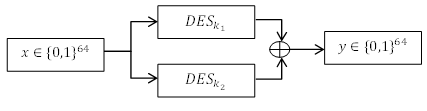
\includegraphics[scale=0.75]{scheme02}}
\end{figure} 
Маємо односторонню функцію.
\item 
Розглянем функцію $y=f(k,M)=E_{k}(M): \mathcal K \times \mathcal M \to \mathcal Y$. Якщо ШТ $Y$ більше
відстані єдиності, то по ШТ $Y$ можно знайти ключ $k$ і ВТ $M$. Але в загальному випадку, це можно зробити
лише овним перебором, а отже маємо односторонню функцію з секретом. 
\end{enumerate}
          % 02
\section{Важкооборотні функції із секретом. Важкооборотна функція RSA}
\begin{flushright}
\emph{(Автор: Олександр Богуцький. Трохи редагувалось.)}
\par \emph{(Версія від 21 січня 2017 р.)}
\end{flushright}

\begin{mydef}
 Важкооборотною функцією із секретом (лазівкою) називається відображення :
\begin{equation}
y = f_{\text{k}}(x): X \rightarrow Y,
\end{equation}
що залежить від параметру k, таке, що:\par
1) $\forall k, x$ існує поліноміальний (ефективний) алгоритм обчислення $y = f_{\text{k}}(x)$. При цьому знати $k$ необов'язково.
\par2) При невідомому $k$ майже для будь-яких $k, y$ не існує поліноміального алгоритму обчислення оберненої функції $f_{\text{k}} ^{-1} (y)$.
\par3) При відомому $k$ існує поліноміальний алгоритм обчислення $f_{\text{k}} ^{-1} (y) \; \forall k, x$.

Під ефективністю алгоритму розуміємо те, що обчислення ведуться за долі секунди. У той час як обчислення неефективних алгоритмів займатимуть мільярди років, а то й більше. 
\end{mydef}

Зауважимо, що функція $y = f_{\text{k}}(x)$ не обов'язково повинна бути бієкцією.

Як і раніше, потужності $X, Y$ дуже великі.

\begin{mydef}
 Важкооборотною функцією із таємницею RSA називається функція 
\begin{equation} \label{eq:3.1} 
y = x ^{e} \bmod n,
\end{equation}
при чому $n = p \cdot q,\; q \neq p$ ~--- великі прості числа, $(e, \varphi(n)) = 1     $. Зазвичай $p = 2p\prime + 1,\; q = 2q\prime + 1$, де $p\prime,\; q\prime$ ~--- прості.
\end{mydef}
Секрет функції RSA: $q, \; p$, а також $\varphi  (n)$.

Розглянемо оцінки складності:
\par1. Для будь-якого $x$ складність обчислення \eqref{eq:3.1} :  $L_{1} \leq 2 \log {n}$.
\par2. При невідомих $q, \; p,\;\varphi  (n)$ складність обчислення оберненої функції (тобто добування дискретного кореня): $L_{2} = O(\sqrt n)$.

Доведено субекспоненційну оцінку складності обернення фунції 
\[ L_{3} = exp\{ (  \mbox{с}_{0} + O(1)) \ln ^{1/2} n (\ln\ln n) ^ {1/2}) \}. \]

Крім того, вважається, але строго не доведено, що можна досягти такої складності обчислення $L_{4} = exp\{ (  \mbox{с}_{0} + O(1)) \ln ^{1/3} n (\ln\ln n) ^ {2/3}) \}$.

\par3. При відомих $p,\;q$ складність обернення $L_{5} \leq 2 \log n$.

Помітимо, що якщо $x \in X = \{ 0, 1, ..., n-1 \}$, то функція RSA \eqref{eq:3.1} ~--- бієкція.

Тепер розглянемо, як будується криптосистема RSA з використанням функції \eqref{eq:3.1}.

\subsection{Побудова криптосистеми шифрування та цифрового підпису RSA користувачем A}

\par1. Вибір великих простих $p,\; q,\; p \neq q$.

\par2. Обчислення $n = p \cdot q, \; \varphi(n)=(p-1)(q-1)$.

\par3. Знаходження $e:\;1<e<\varphi(n),\;(e,\varphi(n))=1$.

\par4. Обчислення $d$ із рівняння $d \cdot e = 1 \bmod \varphi(n)$, тобто $d = e ^{-1} \bmod \varphi(n)$.

\par5. Оголошення відкритого ключа $(n,e)$ для зашифрування повідомлень для користувача $A$ та для перевірки цифрового підпису $A$.
При цьому $d$ ~--- це секретий ключ $A$ для розшифрування шифр текстів, відправлених користувачеві, і для формування цифрового підпису $A$.

Зрозуміло, що $\varphi (n)$ -- теж секрет $A$.

Якщо $\varphi (n)$ відомо, то криптоаналітик складає систему рівнянь з двома невідомими:
\begin{equation*}
\begin{cases}
    n = p \cdot q, \\
    (p-1)(q-1) = \varphi (n)
\end{cases},
\end{equation*}
та розв'язує її.

Обернена до RSA функція обчислюється легко : 
\begin{equation} 
x = y ^{d} \bmod n.
\end{equation}

\subsection{Зашифрування повідомлення користувачем B}

Зашифрування повідомлення $M \; (1<M<n)$ відбувається наступним чином. Користувач, використовуючи відкритий ключ користувача $A$, обчислює : 
\begin{equation}
C = M^e \bmod n.
\end{equation}
Отриманий шифр текст $C$ відправляється користувачеві $A$.

\subsection{Розшифрування шифртексту C користувачем A}

Розшифрувати шифр текст може лише користувач $A$, який знає секретний ключ. Здійснюється це теж всьго лиш в одну операцію : 
\begin{equation} \label{eq:3.2} 
M = C ^ d \bmod n.
\end{equation}

Дане твердження вимагає доведення, оскільки \eqref{eq:3.2} не є очевидним фактом.
\begin{proof}
Для доведення \eqref{eq:3.2} розглянема 3 випадки:
\par1) $(M,n) = 1$.
\par2) $(M,n) > 1, \; M \vdots p, \; M\not\vdots q$.
\par3) $(M,n) > 1, \; M\not \vdots p, \; M \vdots q$.
\\
На практиці, можливий лише перший випадок, оскільки ймовірність того, що $M$ та $n$ не взаємопрості, порядку $1/2^{500}$ (для випадку коли \textsl{n}--1024 біти), що практично дорівнює нулеві.
Звісно, якби така ймовірність була високою, то здійснювалась би атака на взлом. Вибираючи $M$, шукали б НСД, що не дорівнює 1. Тоді за алгоритмом Евкліда, знаходяться $p$ та $q$.\\ 
\textbf{Розглянемо перший випадок}: $(M,n) = 1$. \\
Тоді $C ^ d \bmod n = M ^ {ed} \bmod n$. \\
Оскільки $ed = 1 \bmod \varphi (n)$, то існує таке ціле число $t$, що $ed = t \cdot \varphi (n) + 1 $. \\
Тому $M ^ {ed} \bmod n = M ^ {t \varphi (n) + 1} \bmod n = (M ^ {\varphi (n)}) ^ t \cdot M \bmod n$.\\
 Оскільки за теоремою Ейлера $M ^ {\varphi (n)} \bmod n = 1$, то $(M ^ {\varphi (n)}) ^ t \cdot M \bmod n = M$.\\
\textbf{Випадок 2}.\\
 Розглянемо $C ^ d \bmod q = M ^ {ed} \bmod q = M ^ {(q-1)(p-1) \cdot t + 1} \bmod q = (M ^ {q-1}) ^ {(p-1)t}M \bmod q$.\\ Оскільки $M \not\vdots q$, то $M ^ {q-1} \bmod q = 1$ за малою теоремою Ферма. \\
Отримуємо $(M ^ {q-1}) ^ {(p-1)t} \cdot M \bmod q = M$. $C ^ d \bmod p = M ^{ed} \bmod p$. Оскільки $M \vdots p$, то $M ^{ed} \bmod p = M \bmod p$. У результаті отримуємо співвідношення:
\begin{equation*}
\begin{cases}
    C ^ d \bmod p = M, \\
    C ^ d \bmod q = M
\end{cases}.
\end{equation*}
За китайською теоремою про лишки, отримуємо $C ^ d \bmod n = M$.\\
Міркування щодо випадку 3 аналогічні міркуванням випадку 2.
\end{proof}

\subsection{Задачі цифрового підпису}

Основними задачами цифрового підпису є:

\par1. Підтвердження справжності (цілісності) повідомлення.
\par2. Підтвердження справжності джерела (автора) повідомлення.
\par3. Забезпечення неможливості підробки цифрового підпису.
\par4. Забезпечення неможливості відмови від цифрового підпису.
\par5. Можливість багакратної перевірки цифрового підпису різними користувачами без зміни системи цифрового підпису. 
\par6. Юридична значимість.

\subsection{Цифровий підпис RSA}
Цифровий підпис формується просто. Користувач використовує власний секретний ключ для підпису повідомлення:
\begin{equation}
S = M ^d \bmod n.
\end{equation}
Далі відбувається формування підписаного повідомлення: до $M$ дописується цифровий підпис $S$. Отже, підписане повідомлення виглядає так ~--- $(M, S)$.

Перевірка цифрового підпису користувачем $B$ здійснюється наступним чином: отримане підписане повідомлення $(M, S)$ розбивається за формальними ознаками на $M$ та $S$, і перевіряється рівність 
\begin{equation} \label{eq:3.3} 
S ^ e \bmod n = M.
\end{equation}
Якщо \eqref{eq:3.3} виконується, то цифровий підпис вірний, тобто повідомлення справжнє, відправити та сформувати його міг лише користувач $A$ і ніхто інший. При наявності іншого результату, це свідчитиме про змінене повідомлення або підроблений цифровий підпис.
Якщо нема спотворень, то \eqref{eq:3.3} виконується, оскільки $S ^ e \bmod n = M ^ {ed} \bmod n = M$ (доведення аналогічне попередньому).

Стійкість системи RSA базується на складності задачі факторизації (розклад великих чисел на множники). Якщо модуль $n$ розкладений на множники $q$ та $p$, то можна обернути важкооборотну функцію та взломати RSA, підробити цифровий підпис.

Не доведено, що якщо за шифр текстом в RSA знайдено відкритий текст, то можна розкласти $n$ на множники $p$ та $q$.
          % 03
\section{Складність алгоритмів}
\begin{flushright}
\emph{(Автор: Антон Вихло. Не редагувалось.)}
\par \emph{(Версія від 18 січня 2017 р.)}
\end{flushright}

\emph{Алгоритм} -- загальна послідовна процедура, яка виконує покрокове рішення певної задачі.

\emph{Вхід алгоритму} -- деяка скінченна множина, представлена у визначеній системі кодування даних.

Розмір даних можна оцінювати як число символів вхідних даних у певній системі кодування.

Після зупинки алгоритму, результат роботи представляється набором символів в певній системі кодування.

\emph{Часова складність алгоритму} визначається числом кроків до зупинки(або часу, наприклад, роботи ЕОМ).

\emph{Алгоритм} -- дискретна процедура, в якій проміжні та кінцеві результати змінюються покроково.

\emph{Ємнісна складність алгоритму} оцінюється максимальною кількістю символів, що оброблюються на кожному кроці. При реалізаціїї алгоритмів, наприклад, на ЕОМ, максимальний об'єм необхідної пам'яті.
\begin{center} Формальні теорії алгоритмів \end{center}
\begin{enumerate} 
\item Детерміновані машини Т'юрінга(ДМТ), недетерміновані машини Т'юрінга(НДМТ).
\item Рекурсивні функції.
\item Нормальні алгоритми Маркова.
\item Теория Поста.
\end{enumerate} 

\begin{center} Узагальнений тезис Черча \end{center}


Будь-який интуітивно зрозумілий алгоритм може бути сформульований в будь-якій із теорій 1-4.

Позначення:

 $A_n$ - алгоритм.

$X$ - область визначення алгоритму(вхідні дані, що належать $X$).

$ x\in X, x$ - індивідуальний вхід(дані).

$||x||$ - розмір входу.

$T(n,x), x \in X, n=||x||$ - часова складність алгоритму  $A_n$ .

$S(n,x), x \in X, n=||x||$ - ємнісна складність  алгоритму  $A_n$ .

\emph{Середньою складністю} називається 

$T_{\text{сер.}}(n) = \sum\limits_{x \in X, ||x||=n}^{} p(x)\cdot T(n,x) , x \in X, n=||x||,  p(x)$ - деякий розподіл імовірностей на множині $X$.

\emph{Складністю в найгіршому випадку} називається 

$T_{max}(n) = \smash{\displaystyle\max_{x \in X, ||x||=n}} T(n,x)$.

\begin{center} Асимптотичні оцінки складності \end{center}

\emph{Складність для майже всіх входів} називаєтьсятака оцінка $T_{\text{м.в.}}(n)$, що 

$\forall  \epsilon  \ge 0$ $\exists  n_0$  така, що відносна частина тих входів  $ x \in X, n=||x||$, для яких  $T(n)\hm \ge  T_{\text{м.в.}}(n) \to  0$, при  $n \to \infty $.

Аналогічно визначається $S_{\text{сер.}}(n), S_{max}(n), S_{\text{м.в.}}(n).$

 \begin{mydef} Пролономіальною часовою складністю називається така $T(n)$, що $\exists p(x)$~-- поліном, і $T(n) = \mathcal O (p(n)), n \to \infty$, де пiд $T(n)$ розуміється будь-яка складність  $T_{\text{сер.}}(n), T_{max}(n), T_{\text{м.в.}}(n).$\end{mydef}

 \begin{mydef}Експоненційною часовою складністю називається $T(n) \asymp a^{cn}, a = const \hm \ge 1, c = const \ge 0, n \to \infty$. \end{mydef}

Інше означення $T(n) = \theta (a^{cn}).$

 $T(n) \asymp a^{cn} \Longleftrightarrow  T(n) = \mathcal O (a^{cn})$ і $ a^{cn} = \mathcal O(T(n))$

Інакше $\exists 0 \le c_1 \le c_2 \le \infty$ такі, що $c_1a^{cn}\leq T(n) \leq c_2a^{cn}$

Зазвичай $ 0 \le c \le 1,$ $a = 2; e; 10.$ 

 \begin{mydef} Субекспоненційною оцінкою складності (часової) називається така оцінка  $T(n) \asymp \exp (n^\gamma (\ln n)^{1-\gamma})$, $ 0\leq \gamma \leq 1, n \to \infty$. \end{mydef}

При $\gamma \to 0$ субекспоненційна оцінка наближається до поліноміальної.

При $\gamma \to 1$ субекспоненційна оцінка наближається до експоненціальної.

Аналогічно визначаються поліноміальні, експоненційна та субекспоненційні оцінки $S(n)$.

 \begin{mydef}Класом $P$ називаэться клас задач для яких $\exists$ поліноміальний часовий алгоритм (в найгіршому випадку) на ДМТ рішення задачі. \end{mydef}

 \begin{mydef}Класом $NP$ називається клас задач для яких $\exists$ поліноміальний часовий алгоритм (в найгіршому випадку) на НДМТ рішення задачі. \end{mydef}

Відомо: $P \subseteq NP.$

Не доведено: $ P = NP$ або $NP \backslash P \ne \emptyset$.
          % 04

\chapter{Криптографічні геш-функції та схеми цифрового підпису}

\section{Геш-функції}
\begin{flushright}
\emph{(Автор: Євген Грубіян. Редагувалось.)}
\par \emph{(Версія від 22 січня 2017 р.)}
\end{flushright}

\textit{Геш-функція} - одностороння функція, яка перетворює блок даних довільного розміру в блок даних фіксованого розміру. При цьому прообразів для одного значення геш-функції може бути дуже багато, а знаходження бодай одного із них є дуже трудомістким. Однією із причин розробки геш-функцій стала необхідність підписувати повідомлення довільного розміру та перевіряти цілісність даних.

Геш-функції в криптографії використовується:
\begin{enumerate}
\item Для створення геш-образів для повідомлень цифрового підпису.
\item Для безпечного зберігання паролів.
\item Для автентифікації.
\item В криптопротоколах.
\item Для генерації випадкових послідовностей, функцій, ключів.
\item Для перевірки правильності обчислювальних операцій.
\end{enumerate}

Розглянем варіант цифрового підпису \textit{RSA} без геш-функцій:\\
Нехай абонент \textbf{A} має криптосистему \textit{RSA} з відкритим ключем \( \left( n, e \right) \) і таємним ключем \( d \).
\begin{algorithm}[Цифровий підпис \textit{RSA} без геш-функціїї]\ 
\begin{itemize}
\item \textbf{A} розбиває \( M \) на блоки: \( M = M_1 M_2 \dots M_t \), де \( |M_i|<n,\ i = \overline{1,\ t} \).
\item \textbf{A} обчислює цифровий підпис для кожного із блоків окремо \( S_i = M_i^d\ mod\ n \)
\item \textbf{A} формує підписане повідомлення \( \left(M, S_1 S_2 \dots S_t \right) \)
\end{itemize}
\end{algorithm}
Недоліки цього способу:
\begin{enumerate}
\item Трудоємність.\\
Очевидно, що чим більше блоків необхідно підписати тим більше часу потрібно витратити, тому даний варіант є не практичним з обчислювальної точки зору.
\item Атаки перестановкою і видаленням блоків. \\
Оскільки блоки підписуються незалежно криптоаналітик \textbf{E} може видаляти та переставляти блоки як йому завгодно без порушення правильності підпису, продукуючи повідомлення з вірним цифровим підписом, які \textbf{A} ніколи не підписував і не підписав би. 
\item Комутативні атаки. \\
Нехай \( A \) підписав два повідомлення \( \left( M_1,\ S_1 \right),\ \left( M_2,\ S_2 \right) \). Криптоаналітик \textbf{E} формує неправдиве повідомлення з вірним цифровим підписом \( \left(M_3,\ S_3 \right) \), де \( M_3 = M_1 M_2 \ mod\ n \), \( S_3 = S_1 S_2 \ mod\ n \). Перевірка цифрового підпису цього повідомлення дає \[ S_3^e \ mod\ n = (S_1 S_2)^e\ mod\ n = (M_1^d M_2^d)^e \ mod\ n = M_1^{de} M_2^{de} \ mod\ n = M_1 M_2\ mod\ n = M_3 \]
Тобто підпис правильний. І взагалі кажучи \( \forall (M_i,\ S_i),\ i = \overline{1,\ t} \) повідомлень, які підписав \textbf{A} можна скласти неправдиве повідомлення з вірним цифровим підписом: \( ( \widetilde{M},\ \widetilde{S} ) \), де \[ \widetilde{M} = \left( \prod_{i=1}^t M_i^{\alpha_i} \right) mod\ n,\ \widetilde{S} = \left( \prod_{i=1}^t S_i^{\alpha_i} \right) mod\ n, \ \alpha_i \in \Zring{+} \]
\item Атака з неявним використанням таємного ключа \( d \)\\
Нехай криптоаналітик \textbf{E} хоче щоб \textbf{A} підписав повідомлення \( M \), яке вигідне криптоаналітику. 
\begin{algorithm}[Атака з неявним використанням таємного ключа]\ 
\begin{itemize}
\item \textbf{E} вибирає деяке число \( r \colon gcd(r,n) = 1 \).
\item \textbf{E} обчислює \( \widetilde{M} = r^e M\ mod\ n \).
\item \textbf{E} відправляє повідомлення \( \widetilde{M} \) для цифрового підпису \textbf{A}.
\item Якщо \textbf{A} підписав запропоноване повідомлення \( \widetilde{M} \), \textbf{E} отримує підписане повідомлення \( (\widetilde{M},\ \widetilde{S}) \) та може обчислити підпис початкового вигідного для \textbf{E} повідомлення \( M \):
\[ \widetilde{S} = \widetilde{M}^d\ mod\ n = r^{ed} M^d\ mod\ n = r M^d\ mod\ n\]
\[ S = M^d = \widetilde{S} r^{-1}\ mod\ n \]
\item \textbf{E} формує вигідне для нього підписане повідомлення \( \left( M,\ S \right) \). 
\end{itemize}
\end{algorithm}
\end{enumerate}

Введемо позначення:\\
\( \Zring{2} = \{0, 1\} \) - алфавіт із двох символів.\\
\( \Zring{2}^{*} \) - замикання Кліні алфавіту \( \Zring{2} \) (Множина послідовностей всіх довжин із алфавіту). \\
\( \Zring{2}^{m} \) - множина послідовностей довжини \( m \).

\begin{mydef}
\textit{Геш-функцією} в криптографії називається відображення:\\
\[ h \colon \Zring{2}^{*} \rightarrow \Zring{2}^{m},\ m>1\]
яке має властивості:
\begin{enumerate}
\item \( \forall M \in \Zring{2}^{*} \) обчислення геш-образу \( H = h(M) \) швидке.
\item \( h(x) \) - обчислювально одностороння функція, тобто \( \forall H \in \Zring{2}^{m} \) неможливо знайти хоча б одне \( M \), таке що \( H = h(M) \).\\
\textit{Приклад}\\
\( m=256,\ ||M||=500 \). Тоді в середньому \( \forall H \in \Zring{2}^{m}\ \exists \frac{2^{500}}{2^{256}} = 2^{244} \) можливих \( M \). Тобто знайти таке повідомлення-прообраз випадково неможливо.
\item Геш-функція чутлива до змін входу, тобто має лавинні ефекти.
\item Слабка стійкість до колізій, тобто для кожного фіксованого повідомлення \( M \) неможливо знайти таке \( M' \neq M \) таке, що \( h(M) = h(M') \).
\item Сильна стійкість до колізій, тобто неможливо знайти хоча б одну пару повідомлень \( (M, M') \), таку що \( h(M) = h(M') \)
\end{enumerate}
\end{mydef}

\begin{mydef}
Геш-функція, яка має властивості 1-4 називається \textit{слабкою односторонньою геш-функцією}.
\end{mydef}

\begin{mydef}
Геш-функція, яка має властивості 1-5 називається \textit{сильною односторонньою геш-функцією}.
\end{mydef}

Розглянемо цифровий підпис \textit{RSA} до повідомлення \( M \) будь-якої довжини з геш-функцією \( h(x) \).
Нехай абонент \textbf{A} має криптосистему \textit{RSA} з відкритим ключем \( \left( n, e \right) \), таємним ключем \( d \) і відкриту геш-функцією \( h(x) \colon ||h|| = m,\ 2^{m} < n \).
\begin{remark}
Зазвичай довжина виходу геш-функції \( m \) складає 128, 160, 192, 256 або 512 біт. Найпоширенішими є геш-функції з \( m \) 128, 160, 256. На цих довжинах досягається компроміс між стійкістю до колізій та швидкістю обчислення геш-функції.
\end{remark}
\begin{algorithm}[Цифровий підпис \textit{RSA} з геш-функцією]\ 
\begin{itemize}
\item \textbf{A} обчислює значення геш-функції повідомлення \( M \): \( H = h(M) \)
\item \textbf{A} обчислює цифровий підпис: \( S = H^d\ mod\ n \)
\item \textbf{A} формує підписане повідомлення \( (M,\ S) \).
\end{itemize}
\end{algorithm}
Нехай підписане повідомлення \( (M,\ S) \) перевіряє абонент \textbf{B}.
\begin{algorithm}[Перевірка цифрового підпису \textit{RSA} з геш-функцією]\ 
\begin{itemize}
\item \textbf{B} розбиває \( (M,\ S) \) на \( M \) та \( S \) по формальним ознакам
\item \textbf{B} обчислює \( H = h(M) \)
\item \textbf{B} перевіряє рівність \( S^e\ mod\ n = H \). Якщо вона виконується, то цифровий підпис \textit{вірний}, якщо не виконується, то підпис \textit{не вірний}.
\end{itemize}
\end{algorithm}

Розглянемо можливості атак на цифровий підпис з геш-функцією. Основні атаки базуються на пошуці колізій в використаній геш-функції, тобто фактів однакових геш-значень при різних аругументах геш-функції.\\
Нехай криптоаналітик \textbf{E} намагається отримати вигідне для нього повідомлення з вірним цифровим підписом абонента \textbf{A}. Розглянемо наступні два варіанта атаки:
\begin{enumerate}
\item Якщо \textbf{E} має підписане \textbf{A} повідомлення \( (M,\ S) \)\\
\textbf{E} будує ряд повідомлень \( M_1, M_2, \dots, M_t\colon M_i \neq M \) та обчислює їхні геш-значення \( H_1, H_2, \dots, H_t\colon H_i = h(M_i) \).\\
Пободуємо ймовірнісну модель атаки, в припущенні, що всі геш-значення рівноймовірні на множині \( \Zring{2}^m \). Позначимо \( P_1, Q_1 \) - ймовірності слабкої колізії і відсутності слабкої колізії відповідно. Тоді:
\[ Q_1 = \left(1-\frac{1}{2^m} \right)^t,\ P_1 = 1 - \left(1-\frac{1}{2^m} \right)^t \]
Таким чином асимптотично можна записати:
\[ Q_1 = e^{-t/2^m},\ P_1 = 1-e^{-t/2^m}\ m,t\rightarrow \infty \]
Середня кількість необхідних повідомлень для здійснення атаки знаходженням колізії:
\[ t = 2^m ln\frac{1}{1-P_1} \]
\item Якщо криптоаналітик \textbf{E} не чекає підписаного \textbf{A} повідомлення(\textit{атака Ювала}).\\
\textbf{E} будує ряди повідомлень прийнятних \( M_1, M_2, \dots, M_t \) та неприйнятних \( \widetilde{M_1}, \widetilde{M_2}, \dots, \widetilde{M_t} \) для \textbf{A} повідомлень, тобто таких, які він би підписав і не підписав ніколи відповідно та обчислює їхні геш-значення \( H_1, H_2, \dots, H_t \) та \( \widetilde{H_1}, \widetilde{H_2}, \dots, \widetilde{H_t} \) відповідно. Якщо знайдеться така пара індексів \( (i,\ j) \), що \( H_i = \widetilde{H_j} \), то криптоаналітик \textbf{E} посилає повідомлення \( (M_i,\ H_i) \) для цифрового підпису \textbf{A} та отримавши підписане повідомлення \( (M_i,\ S_i) \) формує неправдиве повідомлення з вірним цифровим підписом \( \left( \widetilde{M_j},\ S_i \right) \).\\
Будуючи ймовірнісну модель по аналогії з попереднім випадком варто зазначити, що в якості ймовірностей \( P_2,\ Q_2 \) варто брати ймовірності сильної колізії та її відсутності:
\[ Q_2 = \left(1-\frac{1}{2^m} \right)^{t^2},\ P_2 = 1 - \left(1-\frac{1}{2^m} \right)^{t^2} \]
Варто зазначити що при однаковому \( t \) ймовірність сильної колізії більша за ймовірність слабкої. \\
Середнє число повідомлень для успішної атаки складатиме:
\[ t = 2^{m/2} \sqrt{ln\frac{1}{1-P_2}} \]
\end{enumerate}
          % 05
\section{Загальні схеми побудови геш-функцій. Характеристики відомих геш-функцій. Цифровий підпис Ель-Гамаля.}
\begin{flushright}
\emph{(Автор: Яна Євсюкова. Редагувалось.)}
\par \emph{(Версія від 22 січня 2017 р.)}
\end{flushright}

\subsection{Загальні схеми побудови геш-функцій.}
Геш-функція необхідна для того, щоб перетворювати послідовність будь-якої довжини в зазначену. Існує декілька схем побудови геш-функції:
\subsubsection*{Схема l. Побудова геш-функції}
Нехай \textit{M}--відкритий текст. Відкритий текст розбивається на блоки \textit{$M=M_1M_2\ldots M_t$}. Довжина \textit{$M_i$}--ого блоку дорівнює \textit{m} біт, де \textit{$i=\overline{1,t}$}.\\
Будується функція стиснення. Зазвичай дана функція є односторонньою, що володіє лавинним ефектом та іншими характеристиками. Причому можна брати вже відомі нам односторонні функції. Наприклад, функція Діффі-Гелмана, RSA, тобто ті функції, що використовуються в асиметричній криптографії з відкритими ключами. Однак, в стандартних геш-функціях, вони зазвичай не використовуються, оскільки працюють досить повільно.\\
Функції стиснення будуються завдяки деяким стандартним операціям: \textit{XOR, додавання за модулем, циклічний зсув, логічні операції} та інші.\\
Наприклад,\\ \textit{$$(n,m)-f$$} функція, на вході якої \textit{n} біт, а на виході \textit{m} біт.\\
Далі, по рекурентній процедурі обчислюється $$H_i=F(M_i \oplus H_{i-1}), \textit{$i=\overline{1,t} \: ,$}$$
де \textit{$H_0$} початковий вектор (зазвичай, відкритий).\\
Останній блок \textit{$H_t$} -- це вихідне значення геш-функції \textit{$h(x)$}.$$H_t=h(M)$$
Тобто дана процедура є покрокова. На кожному кроці оброблюється один блок відкритого тексту \textit{M} та весь час замішуються попередні результати з наступними блоками. І в останньому значенні \textit{$H_t$} будуть замішані всі біти повідомлення.\\
Існує й інша процедура гешування. Наприклад, 
\textit{$$(2m,m)-f$$}функція, на вході якої \textit{2m} біт, а на виході \textit{m} біт.\\
Тоді функція \textit{$H_i$} будується наступним чином:
$$H_i=F(M_i , H_{i-1}), \textit{$i=\overline{1,t} \:.$}$$

\subsubsection*{Схема ll. Побудова геш-функції}
Нехай \textit{M}-відкритий текст. Відкритий текст розбивається на блоки \textit{$M=M_1M_2\ldots M_t$}, \textit{$\left\|M_i\right\|=m$} біт, \textit{$i=\overline{1,t}$}.\\
Нехай, відповідно \textit{$E_k(x)$}--алгоритм блочного шифрування. При цьому розмір входу, виходу та ключа однакові (m біт).
\textit{$$\left\|E_k \right\| = \left\| k \right\| = \left\| x \right\| = m $$}
Тоді, відповідно, рекурентно обчислюється:
$$H_i=E_A(B) \oplus C, \textit{$i=\overline{1,t}\: ,$}$$
де \textit{A,B,C}-\textit{m}-вимірні вектора.\\
\textit{A,B,C} можуть приймати одне із значень:
\begin{enumerate}
        \item значення блоку \textit{$M_i$}
        \item значення попереднього гешу \textit{$H_{i-1}$}
        \item $M_i \oplus H_{i-1}$
        \item $D=const$ - \textit{m}-вимірний вектор
\end{enumerate}
Усього отримаємо 64 можливих варіанти (на кожен із трьох векторів маємо по чотири можливих значення, тобто $4^3=64$). $52$ з них признані слабкими, тому використовують лише $12$ останніх варіантів.\\
Наприклад,
\begin{enumerate}
        \item $H_i=E_{M_i}(M_i) \oplus H_{i-1}$
        \item $H_i=E_{H_{i-1}}(M_i) \oplus M_i$
        \item $H_i=E_{M_i}(M_i \oplus H_{i-1}) \oplus H_{i-1}$
        \item $H_i=E_{H_{i-1}}(M_i \oplus H_{i-1}) \oplus M_i$
\end{enumerate}
Вихідним значенням геш-функції \textit{$h(M)$} є останній блок.$$h(M)=H_t$$
\subsection*{Характеристики відомих геш-функцій.}
Розглянемо випадок, коли геш-функції побудовані по \textbf{Схемі l}, тобто, коли використовується не шифратор, а лише бінарні операції.
\begin{enumerate}
        \item Автором перших геш-функцій,що використовувались, став Рівест (один з авторів RSA). Ним були створені такі геш функції:
        \begin{enumerate}
                \item[] \textit{MD2} (1989р.)
                \item[] \textit{MD4} (1990р.)
                \item[] \textit{MD5} (1991р.)
        \end{enumerate}
        Вихідна строка даних геш-функцій складає $128$ біт, що зараз є недодтатнім для використання.\\
        Геш-функція \textit{MD2} майже не використовувалась. Вона створена для 8-розрядних процесорів, а \textit{MD4} та \textit{MD4} для 32-розрядних процесорів.\\
        При цьому, коли запропонували геш-функцію \textit{MD4}, майже одразу було знайдено вразливості з точки зору побудови колізій. Тому Рівест трохи ускладнив функцію та отримав \textit{MD5}. Вона працює повільніше, ніж \textit{MD4}, однак знайдена колізія була усунена. Після чого \textit{MD5} років 20 була найпопулярнішою геш-функцією, але зараз вона знімається з використання.
        \item \textit{SHA-1} - стандарт США (1995р).\\
        \textit{SHA-1} використовувалсь у стандарті цифрового підпису \textit{SHS}.\\
        Вихідна строка даної геш-функцій складає $160$ біт.\\
        Функції стиснення в пункті 1 та пункті 2 будувалися чергуванням операцій XOR, циклічного сзуву, додавання за модулем $2^{32}$, логічних операцій AND та OR. Чергуя дані операції, будувалась функція, яка обчислювально була одностороння та володіла гарними властивостями перемішування.
        \item Переможець конкурсу \textit{SHA-3} (2007-2012рр.).\\
        В 2010 році на конкурсі було відібрано 14 кандитатів на перемогу. А в 2012 році проголосили переможця. Ним став \textit{Кесеак} з вихідною строкою у $256$ біт.
\end{enumerate}
Розглянемо випадок, коли геш-функції побудовані по \textbf{Схемі ll}, тобто, коли використовується шифратор.
\begin{enumerate}
\item \textit{ГОСТ Р 34-11} (1994р.).\\
В Україні є стандартом з 1995 року. Також є стандартом Россії та деяких держав СНД.\\
Вихідна строка даної геш-функцій складає $256$ біт.\\
Для побудови функції стиснення використовується шифр \textit{ГОСТ Р 28147-89}.\\
Довгочасні ключі фіксуються(декілька варіантів на вибір).
\end{enumerate}
Таким чином, усі зазначені геш-функції є функціями без секрету, тобто кожен може використовувати їх.
\subsection*{Цифровий підпис Ель-Гамаля.}
Більшість європейских держав будують сучасний цифровий підпис за схемою Ель-Гамаля. Розглядатиметься базовий варіант підпису Ель-Гамаля, в той час як існують сотні варіантів даного цифрового підпису. Вони мають однакову односторонню функцію що визначає стійкість, а саме функцію Діффі-Геллмана. Стійкість цифрового підпису Ель-Гамаля побудована на складності залачі дискретного логарифмування. Побудова підпису подібна до схеми шифрування Ель-Гамаля.\\
\subsubsection*{Побудова схеми цифрового підпису Ель-Гамаля користувачем \textbf{А}:}
\begin{enumerate}
\item \textbf{А} обирає велике просте число \textit{p} та примітивний елемент $\alpha$ поля \textit{$F_p$}, де \textit{$p$} та $\alpha$ не є секретними.
\item \textbf{А} обирає секретний ключ \textit{k} та обчислює: $$y=\alpha^{k}mod p$$ Також обирається геш-функція \textit{h(x)}.
\item \textbf{А} оголошує відкритий ключ \textit{$(p,\alpha,y)$} для перевірки цифрового підпису. Секретний ключ \textit{k} створений для формування цифрового підпису.
\end{enumerate}
\subsubsection*{Формування цифрового підпису до повідомлення \textit{M} довільної довжини з геш-функцією користувачем \textbf{А}}
\begin{enumerate}
\item \textbf{А} обирає випадковий параметр цифрового підпису \textit{$x_M$} (для кожного попідомлення \textit{$M$} параметр обирається знову), $1<x_M<p-1$, gcd$(x_M,p-1)=1$.\\
 Обчислюється $$r=\alpha^{x_M}mod p$$
\item Знаходимо розв'язок рівняння відносно \textit{$S$}: $$H=kr+x_{M}Smod(p-1) \: ,$$ 
де $H=h(M)$, тобто $$S=(H-kr)x^{-1}_{M}mod (p-1)$$ 
\item \textbf{А} формує підписане повідомлення \textit{$(M,r,S)$} де \textit{$(r,S)$} є цифровим підписом.
\end{enumerate}
\subsubsection*{Перевірка цифрового підпису користувачем \textbf{B}}
\begin{enumerate}
\item Користувач \textbf{B} ділить повідомлення на три частини:$$(M,r,S)\rightarrow M,r,S$$
\item Обчислює \textit{$h(M)=H$}
\item Перевіряє рівність: $$?y^rr^Smodp=\alpha^H?$$
Якщо рівність виконується, то підпис вірний, і навпаки, якщо рівність не виконується, то підпис хибний.\\
Дійсно, якщо спотворення відсутні, то виконується: $$y^rr^Smodp=\alpha^{kr+x_{M}S}modp=\alpha^{t(p-1)+H}modp=(\alpha^{p-1})^t\alpha^{H}modp=\alpha^{H} \: ,$$
де $(\alpha^{p-1})modp\equiv1$ за малою теоремою Ферма.
\end{enumerate}
\textit{\textbf{Зауваження!}} Під час формування цифрових підписів різних повідомлень \textit{$M_1$} та \textit{$M_2$}, парметри цифрового підпису \textit{$x_{M_1}$} та \textit{$x_{M_2}$} не мають співпадати.\\
Нехай \textit{$x_{M_1}=x_{M_2}$}. Криптоаналітик може виконати успішну атаку, оскільки він має: $$(M_1,r_1,S_1)=(M_2,r_2,S_2)$$
Криптоаналітик помічає, що \textit{$r=r_1=r_2=\alpha^{x}modp$}, тобто \textit{$x_{M_1}=x_{M_2}$} та складає систему рівнянь:
$$h(M_1)=H_1=kr+xS_1mod(p-1)$$
$$h(M_2)=H_2=kr+xS_2mod(p-1)$$
Відповідно, криптоаналітик знаходить секретний ключ \textit{k} та параметр \textit{x}. Таким чином, система повністю зламана.
          % 06
\section{Одностороння функція Рабіна з секретом}
\begin{flushright}
\emph{(Автор: Антон Карпець. Трохи редагувалось.)}
\par \emph{(Версія від 19 січня 2017 р.)}
\end{flushright}

\subsection{Визначення}

\begin{mydef}
Односторонньою функцією Рабіна називається функція: 
\begin{equation} \label{eq:7.1}
y = x ^{2} \bmod n,
\end{equation}
де $n = p \cdot q,\; p \neq q$ ~--- великі прості числа. Секретом функції Рабіна є числа $p$ та $q$.
\end{mydef}

\begin{remark}
Одностороння функція Рабіна не є частковим випадком односторонньої функції RSA ($y = x ^{e} \bmod n$,
$n = p \cdot q,\; p \neq q$ ~--- великі прості числа), оскільки в схемі RSA $(e, \varphi(n)) = 1$, тобто, $(e, (p-1)(q-1)) = 1$. Це означає, що $e$ не ділиться націло на 2.
\end{remark}

\begin{remark}
Функція Рабіна не є бієкцією на множині $X = \{ 0, 1, ..., n-1 \}$ на відміну від RSA, яка є бієктивним відображенням на множині $X$. Окрім того, значення даної функції є квадратичними лишками, якщо $(x, n) = 1$.
\end{remark}

\begin{remark}
Функція, обернена до функції \eqref{eq:7.1} - $y ^{\frac{1}{2}} \bmod n$, яка називається дискретним добуванням квадратного кореня, обчислюється лише для тих $y$, які є квадратичними лишками і не є однозначною.
\end{remark}

\subsection{Складність обчислень}

\par1. Для $\forall x \in X = \{ 0, 1, ..., n-1 \}$ обчислення $y = x ^{2} \bmod n$ потребує однієї операції піднесення до квадрату за модулем $n$.
\par2. Секретом функції Рабіна є числа $p$ та $q$. Тому, коли вони відомі, то обернення функції \eqref{eq:7.1} (отримання значення оберненої до $y$ функції $y ^{\frac{1}{2}} \bmod n$) обчислюється за
\begin{equation} \label{eq:7.2} 
L_1 = O(\log{n})
\end{equation}
операцій піднесення до квадрату та множення за модулем $n$.
\par3. У випадку, коли розклад $n = p \cdot q$ невідомий, то складність обернення становить
\begin{equation} \label{eq:7.3}
L_2 = O(\exp{(\ln{\frac{1}{2}} \cdot n \cdot (\ln{\ln{n}})^{\frac{1}{2}})}),
\end{equation}
що є доведено, або
\begin{equation} \label{eq:7.4}
L_3 = O(\exp{(\ln{\frac{1}{3}} \cdot n \cdot (\ln{\ln{n}})^{\frac{2}{3}})}),
\end{equation}
що припускається.

\begin{algorithm}{Обернення функції Рабіна при відомому розкладі $n = pq$}
\par1. Обчислення $y ^{\frac{1}{2}} \bmod p$, де p - просте число.
Існує три можливі випадки:
\begin{itemize}
        \item $p=4m+3$,
        \item $p=8m+5$,
        \item $p=8m+1$, де $m \in \mathbb{Z}$.
\end{itemize}

Нехай $p=4m+3$, $y$ - квадратичний лишок. Тоді справедлива наступна рівність: $y^{\frac{p-1}{2}}=1 \bmod p$, звідки маємо, зважаючи на вигляд числа $p$, що $y^{2m+1}=1 \bmod p$. Домноживши на $y$ та взявши квадратний корінь з обидвох сторін, маємо: $y ^{\frac{1}{2}} = \pm y^{m+1} \bmod p$.

Нехай $p=8m+5$, $y$ - квадратичний лишок. Тоді справедлива наступна рівність: $y^{\frac{p-1}{2}}=1 \bmod p$, звідки маємо, зважаючи на вигляд числа $p$, що $y^{4m+2}=1 \bmod p$. Добувши квадратний корінь, отримуємо: $y^{2m+1}= \pm 1 \bmod p$. У випадку, коли $y^{2m+1}=1 \bmod p$, маємо: $y ^{\frac{1}{2}} = \pm y^{m+1} \bmod p$. 
\begin{remark}
2 - квадратичний нелишок за модулем $p=8m+5$, оскільки $\Legendre{2}{p} = (-1)^{\frac{p^2-1}{8}}=-1$. Тоді $2^{\frac{p-1}{2}}=2^{4m+2}=-1\bmod p$
\end{remark}
У випадку, коли $y^{2m+1}=-1 \bmod p$, домноживши дане рівняння на $2^{4m+2}=-1\bmod p$, отримуємо: $y^{2m+1} \cdot 2^{4m+2}=1 \bmod p$. Таким чином, $y ^{\frac{1}{2}} = \pm y^{m+1} \cdot 2^{2m+1} \bmod p$.

Нехай $p=8m+1$, $y$ - квадратичний лишок. Тоді справедлива наступна рівність: $y^{\frac{p-1}{2}}=1 \bmod p$, звідки маємо, зважаючи на вигляд числа $p$, що $y^{4m}=1 \bmod p$, що рівносильно: $y^{2m}= \pm 1 \bmod p$. Далі шукається квадратичний нелишок $a$, який використовується декілька разів в рівняннях для отримання (+1) в правій частині (аналогічно попередньому випадку).

\begin{remark}
Якщо $p=4m+3$, то $p$ називається простим числом Блюма. Якщо $n = p \cdot q, p=4m+3, q=4k+3$, то число $n$ називається числом Блюма.
\end{remark}

\par2. Обчислення $y ^{\frac{1}{2}} \bmod q$, де q - просте число - аналогічно першому пункту.

\par3. Обчислення $y ^{\frac{1}{2}} \bmod n$, де $n = p \cdot q, p\neq q$ (власне, обернення функції Рабіна)

Оскільки $p\neq q$, то $(p, q) = 1$. Тоді маємо систему:
\begin{equation*}
\begin{cases}
y^{\frac{1}{2}}=\beta_p \bmod p,\\
y^{\frac{1}{2}}=\beta_q \bmod q.
\end{cases}
\end{equation*}
За китайською теоремою про лишки: $y^{\frac{1}{2}} \bmod n = [\pm\beta_p \cdot q \cdot (q^{-1}\bmod p) \pm \beta_q \cdot p \cdot(p^{-1} \bmod q)]\bmod n$.
\end{algorithm}

\begin{algorithm}{Факторизація n = pq при відомих чотирьох коренях функції Рабіна}
Маємо функцію Рабіна $y = x ^{2} \bmod n$, де $n = p \cdot q,\; p \neq q$. Нехай відомі її корені $x_1, x_2, x_3, x_4$. Знайдемо серед них такі два корені $x_i$ та $x_j$, що $x_i \neq \pm x_j$. Маємо систему:
\begin{equation*}
\begin{cases}
        x^2_i = y \bmod n,\\
        x^2_j = y \bmod n
\end{cases}.
\end{equation*}
Віднявши від верхньої частини нижню, маємо: $(x_i-x_j)(x_i+x_j) = 0 \bmod n$. Але $(x_i-x_j) \not\vdots n$ та $(x_i+x_j) \not\vdots n$. Отже, $(x_i+x_j, n) = p$ або $(x_i+x_j, n) = q$.
За алгоритмом Евкліда знаходимо $p$ або $q$ та, відповідно, $q = \frac{n}{p}$ або $p = \frac{n}{q}$.
\end{algorithm}
\begin{claim}
Задача добування квадратного кореня в функції Рабіна $y = x ^{2} \bmod n$, де $n = p \cdot q,\; p \neq q$, поліноміально еквівалентна задачі факторизації $n = pq$.
\end{claim}          % 07
\section{Системи шифрування та цифровий підпис Рабіна}
\begin{flushright}
\emph{(Автор: Маша Коляда. Редагувалось)}
\par \emph{(Версія від 22 січня 2017 р.)}
\end{flushright}

Дана система шифрування та цифрового підпису використовує односторонню функцію Рабіна : $y=x^2 \bmod n$, де $n=p \cdot q$, $p\ne q$ -- великі прості числа.

\textit{Побудова системи шифрування Рабіна користувачем А}:
\subsection{Схема шифрування Рабіна 1}

\begin{center}
 \textbf{Зашифрування відкритого тексту користувачем \textsl{B}}
\end{center}

\begin{enumerate}
        \item Користувач \textsl{А} обирає прості числа $p,q : p\ne q$. Зазвичай $p=2 \cdot p’+1$,  $q=2 \cdot q’+1$, де $p’, q’$ -- великі прості числа.
        \item Користувач \textsl{А} обчислює $n=p \cdot q$, де $p, q$ -- його секретний ключ.
        \item Користувач \textsl{A} \textit{«оголошує»} відкритий ключ $n$ для зашифрування повідомлень до нього.
        \item Зашифрування повідомлення \textsl{M} користувачем \textsl{B}: $ C=M^2 \bmod n$ – шифртекст, \par
         де $\sqrt{n}<M<n$.
        \item Користувач \textsl{B} відправляє повідомлення користувачу \textsl{А}.    
\end{enumerate}
\textbf{Зауваження}:  При $M^2<n$, розрахунок квадратного кореня аналогічний до розрахунку квадратного кореня на множині дійсних чисел, що легко виконується.\\

\begin{center}
\textbf{Розшифрування шифртексту користувачем  \textsl{А}}:
\end{center}

\begin{enumerate}
        \item   Використовуючи $p$, обчислює: $\pm \beta_p=C^{\frac{1}{2}}\bmod p$.
        \item Використовуючи $q$, обчисює: $\pm \beta_q=C^{\frac{1}{2}}\bmod q$.
        \item За китайською теоремою про лишки знаходить 4 корені:
        \[
         C^{\frac{1}{2}}\bmod n={(\pm \beta_p)\cdot q \cdot q^{-1}\bmod p 
         \pm \beta_q \cdot p \cdot p^{-1}\bmod q}.
        \]
        Отримує  ${M_1,M_2,M_3,M_4}$, після чого обирає один з цих коренів за змістом.   
\end{enumerate}


\subsection{Схема шифрування Рабіна 2(коли n – число Блюма)}

\begin{center}
 \textbf{Зашифрування  відкритого тексту $M$ : $\sqrt{n}<M<n$ користувачем \textsl{В}}
\end{center}
\begin{enumerate}
        \item Обчислює $M^2\bmod n=C$.
        \item Обчислює 2 біти: 
\begin{align*}
      b_1 &= \begin{cases}
        0, &\text{якщо \textsl{M} парне} \\
        1, &\text{інакше}
        \end{cases}  \\
      b_2 &=  \begin{cases}
         0, &\text{якщо} \left(\frac{M}{n}\right)=-1\\
         1, &\text{якщо} \left(\frac{M}{n}\right)=1
        \end{cases}
\end{align*}
        %\todo{(ПОМИЛКА. Оточення cases не працює в цьому фрагменті -- розібратись. -- С.Я.)}
        \item Формує зашифроване повідомлення $(C,b_1,b_2)$ та відправляє його користувачу \textsl{А}.   
\end{enumerate}

\begin{center}
 \textbf{Розшифрування  $(C,b_1,b_2)$ користувачем  \textsl{А}}
\end{center}

\begin{enumerate}
        \item  Аналогічно схемі шифрування Рабіна 1 знаходить ${M_1,M_2,M_3,M_4}$.
        \item Використовуючи $(b_1,b_2)$,  обчислює $ (b^i_1, b^i_2) , i=\overline{1,4}$ та обирає $M_i$ у якого $(b^i_1, b^i_2)= (b_1,b_2)$.    
\end{enumerate}
\ Стійкість до атаки на основі шифртексту повністю заснована на(еквівалентна) складності задачі факторизації. Схеми шифрування Рабіна 1 і 2 не стійкі до атаки на основі вибраного шифртексту.

\subsection{Атаки на схеми шифрування}
\begin{center}
\textbf{Атака на схему шифрування Рабіна 1}
\end{center}

\begin{enumerate}
        \item Криптоаналітик \textsl{Е} підбирає послідовність
        відкритого тексту $M_1$….$M_k$, обчислює відповідні їм  $C_1$…$C_k$.
        \item Відправляє отриманий шифртекст \textsl{A}.
        \item  $A$ : $M'_1$….$M'_k$. Перевіряє $M_i=\pm M'_i$.
        \item Якщо така пара знайшлась, то обчислює $\left(M_i\pm M'_i,n\right)=p \: \text{або} \:q$.     
\end{enumerate}

\begin{center}
\textbf{Атака на схему шифрування Рабіна 2}
\end{center}

\begin{enumerate}
        \item  Криптоаналітик \textsl{E} обирає відкритий текст \textsl{M}. Обчислює ($b_1,b_2$).
        \item Обчислює $M^2\bmod n=C$.
        \item Відправляє шифртекст ($C, b_1,b^{'}_2$), де $b^{'}_2=b_2 \oplus 1$
        \item Отримавши відкритий текст $M^{'}$, знає, що $M\ne M^{'}$, обчислює $\left(M_i\pm M^{'}_i,n\right)=p \: \text{або} \: q$.
\end{enumerate}


\subsection{Схема цифрового підпису Рабіна}

\begin{center}
\textbf{Побудова схеми цифрового підпису Рабіна користувачем А}
\end{center}

\begin{enumerate}
        \item Обирає великі прості числа $p,q$ : $p\ne q$.
        \item Обчислює геш-функцію $h(x)$.
        \item Оголошує $n=p \cdot q$.
        \item Оголошує відкритий ключ ($n, h(x)$) для перевірки цифрового підпису \textsl{А}.     
\end{enumerate}
\ При цьому $p,q$ -- секретний ключ користувача \textsl{А} для формування цифрового підпису.

\begin{center}
\textbf{Формування цифрового підпису А}
\end{center}

\begin{enumerate}
        \item   $M =m_1m_2…m_k$. Генерує випадкову послідовність $R=r_1…r_s$.
        \item   Обчислює $h(M||R)=h(m_1…m_k+r_1…r_s)=H$
        \item Перевіряє, чи є $H$ квадратичним лишком за модулем $n$.
        \begin{enumerate}
                \item Якщо виконується $H^{\frac{p-1}{2}}\bmod p=1$ і $H^{\frac{q-1}{2}}\bmod q=1$, переходимо до кроку 4.
                \item інакше переходимо до кроку 1.
        \end{enumerate}
\ Якщо n--число Блюма, то в средньому, цей пункт виконується на 4-ій спробі.
    \item       Обчислює $H^{\frac{1}{2}}\bmod n$:
    \begin{enumerate}
    \item       Використовуючи $p$ обчислює: $\pm \beta_p=H^{\frac{1}{2}}\bmod p$
    \item Використовуючи $q$ обчислює: $\pm \beta_q=H^{\frac{1}{2}}\bmod q$
    \item   За китайською теоремою про лишки знаходить 4 корені: 
\[    
    C^{\frac{1}{2}}\bmod n={\pm \beta_p \cdot q \cdot q^{-1}\bmod p \pm ( \beta_q) \cdot p \cdot p^{-1}\bmod q} \rightarrow M_1,M_2,M_3,M_4
\]
\end{enumerate}
   \item Обирає один з коренів $\beta$, та формує підпис ($M,R, \beta$)
\end{enumerate}

\begin{center}
\textbf{Перевіка цифрового підпису користувачем В}
\end{center}

\begin{enumerate}
        \item   $(M,R,\beta) \rightarrow M,R,\beta$
        \item Обчислює  $h(M||R)=h(m_1…m_k+r_1…r_s)=H$
        \item Перевіряє рівність : $\beta^2 = H \bmod n$.
        \begin{enumerate}
                \item Якщо виконується, то підпис правильний
                \item Інакше, не правильний.
        \end{enumerate} 
\end{enumerate}
\ Складність взлому цифрового підпису Рабіна поліноміально еквівалентна складності задачі факторизації.          % 08

\chapter{Криптосистеми на еліптичних кривих}

\section{Криптосистемы на эллиптических кривых}
\begin{flushright}
\emph{(Автор: Семен Лигін. Російською мовою. Не редагувалось.)}
\par \emph{(Версія від 18 січня 2017 р.)}
\end{flushright}


На эллиптические системы переносятся только задачи, основанные на задаче дискретного логарифма

\begin{equation}
    y= \alpha^x mod p
\end{equation}
где $\alpha$ - примитивный элемент над $F_p$

Недостатки: зыбкость теоретического обоснования, медленная работа. 

Первое понятно, по поводу второго: вот временн\'{а}я сложность. 
    $$T(n) = e^{cn^\nu(logn)^{1-\nu}}$$
    $$0<=\nu<=1$$
    $$\nu=0:$$
    $$T(n) = e^{clogn}=n^c$$
    $$\nu = 1:$$
    $$T(n) = e^{cn}$$
Если строго от 0 до 1 - то такие алгоритмы субэкспоненциальные
Вообще ню примерно равно 1/3
В связи с этим создатели криптосистемы вынуждены увеличивать длину ключа, что не ускоряет работу системы. 
Сейчас длина ключи порядка 2048 бит. 

В 1985 году Миллер и Коблитц предложили строить криптосистемы на эллиптических кривых. А именно: было предложено задавать на эллиптических кривых аддитивную абелеву группу. Собственно:

E - эллиптическая кривая,
P - точка кривой большого порядка, под порядком имеем в виду порядок в группе.

$Q=xP=\underbrace {P+...+P}_{\text x}$

И зная P, Q и E, затруднительно найти Х.

Мультипликативная группа всегда циклична. А группа точек в Е - ваще хз какая, любая может быть. Но это нормально. 

Кстати, $\alpha$ - не обязательно должно быть примитивным элементом. Альфа должно иметь такой порядок, что невозможно создать таблицу для всех степеней $\alpha$, примитивно говоря. В конечном поле легко найти нужные элементы, вот их и берём. 
На практике берём кривые, порядки которых делятся на большое, просто n.

То есть, точки порядка эн. 

и: 
$P, 2P, 3P, ... , nP = O_e$ 

- получается циклическая группа. 

А это - задача дискретного логарифма (найти x по P,Q,E)

Задача дискретного логарифма на эллиптических кривых труднее, чем в конечном поле. Там мы работаем с простыми числами и неприводимыми полиномами, а на эллиптических кривых такого нет, следовательно, криптосистемы на эллиптических кривых при той же длинне ключа l более стойкие, чем в конечном поле. 

В конечном поле ключи длины около 1024B, на ЭК - порядка 160B.

Но не всё так просто. В частности, схема Диффи-Хеллмана не переносится на ЭК тривиально, есть проблемы. 

Вот есть алгоритм Диффи-Хеллмана:

A и B выбрали себе $p$ и $\alpha$ - примитивный элемент $F_p$

$1 < K_A < p-1$

$1 < K_B < p-1$

$y_A = \alpha^{K_A} mod p   -> y_A^{K_B}mod p = \alpha^{K_A * K_B} = K$

И в то же время B:

$y_B = \alpha^{K_B} mod p   -> y_B^{K_A}mod p = \alpha^{K_A * K_B} = K$

И получают одинаковое K.

На эллиптических кривых он же:

$F_q, E, P: ord P = n$

$1 < K_A < n$

$1 < K_B < n$

$Q_A = \alpha^{K_A}*P   -> y_{K_B}*Q_A = K_A * K_B * P = K$

$Q_B = \alpha^{K_B}*P   -> y_{K_A}*Q_B = K_A * K_B * P = K$

Кажется, что они тривиально переносятся. Но есть проблемы. 

КС на ЭК были предложены в 1985 году, но стандарты на них появились около 1999 года. 
Вот в схеме Диффи-Хеллмана: выбираем E, в которой есть точка большого порядка. А как выбрать-то?Нельзя просто посчитать руками. 

Есть алгоритм Скуффа(Schoof)

$P \in Poly$, но если кривая над $F_q$, то $O((log9)^9)$

Многовато.

Также известно неравенство Хассе для определения порядка эллиптической кривой. 
\begin{theorem}[Неравенство Хассе]

Пусть N - порядок эллиптической кривой. 

E - кривая над $F_q$

Тогда
$$ q+1-2*(q)^{-1/2}<=N_E<=q+1+2*(q)^{-1/2} $$
\end{theorem}

\begin{proof}
Поле берём характеристики не два и не три. Подставляем Х и смотрим на квадратичный вычет. 

В среднем половина вычетов и половина невычетов. 

Это $q/2$, в каждом есть по $2y$ - это единица, и $2q^{1/2}$ - это дисперсия.

\end{proof}

Есть масса способов получить одну любую ЭК, например:

$y^2 = x^3 + ax + b$ над $F_q, a,b \in F_q$

Кривую рассмотрим над ${F_q}^n$
Правда, и кривая тогда имеет больше точек. 

Рассмотрим такую кривую. В неравенстве Хассе числа в промежутке лежат очень узко (в каком-то смысле, мне непонятном)

Пусть N - число из интервала, заданного неравенством Хассе. 
Пусть $N_1$ - порядок кривой с A и B.

\begin{table}[]
    \centering
    \begin{tabular}{c|c}
        $W F_Q {F_Q}^2 ... {F_Q}^r$ \\
        $   N_1 N_2 .....N_r$
    \end{tabular}
    \caption{Такую табличку строим}
    \label{tab:my_label}
\end{table}

И есть итеративные формулы, чтобы считать $N_i$ из $N_j$.

Нашли $N_1$, по нему считаем $N_2$ и проверяем, что $N_2$ делит $P$, где P - большое простое число.

Чуть-чуть подробнее об этой проверке. "При помощи кофактора, С - маленькое $z^*$"

Число делим на маленькие числа и затем проверяем на простоту. 
Да - ок. 
Нет - берём следующее число. 

Перебирая находим кривую из $F_q$, и на ${F_q}^n$ будет тот же порядок. 

Теперь ещё раз. Есть уравнение кривой. Рассмотрим её над $F_q$. А надо построить над ${F_q}^n$. 

$$y^2 = x^3 + ax + b$$
$$F_q \to {F_q}^r$$

Знаем, что 
$$ q+1-2*(q)^{-1/2}<=N_E<=q+1+2*(q)^{-1/2} $$

И что:
$$N_1 \to N_2 \to N_3 \to ... \to N_r$$

W - первое число из ***. Оно соответствует какой-то кривой. 

Считаем $N_r$

Проверяем, делится ли $N_r$ на большое простое число. 

Также следует понимать, что в маленьком поле мы можем просто непосредственно посчитать порядок кривой. 

Схема шифрования Эль-Гамаля

Обычно:

$A: p, \alpha$

$1<k<p-1$ - секретный ключ

$y = \alpha^k mod p$ - открытый ключ

$B: m<p$

$1 < X_m < p-1$ - генерится каждый раз заново

$С_1 = \alpha^{X_m} mod p$

$С_2 = y^{X_m}*m mod p$

$B: (C_1, C_2) -> A $

$A: (C_1 ^ {-k} * C_2 = \alpha^{-k*X_M} * \alpha^{k*X_m}*m mod p = m$

На эллиптических кривых есть проблема: мы шифруем точку эллиптической кривой, а надо шифровать число. И нет такого детерменированного алгоритма, который сможет их сопоставить. 

$$ 0 < m < M $$

Пусть - над полем характеристики q, не 2 и не 3. 

M-1 - значение наибольшего сообщения. 

$ M - 1 < q$

$k : 1/{2^k}$ - вероятность не сопоставить точку. 

Каждому M можем сопоставить отрезок. Берём точку и подставляем правую часть ($x^3+ax+b$)

Это и будет точкой эллиптической кривой $m -> P_m$

Если квадратичный невычет - то берём следующее число в этом отрезке. 

И тогда: пусть $1/2$, что квадратичный вычет.

Тогда $1/2^k$ - вероятность не найти. Это ок. 

$A: F_q, E, P$(большого порядка),$ord P = N$
$0<k<n$ - k - секретный ключ. Q - открытый ключ, $Q = k*P$

$B: 0 < X_m < n, m -> P_m$,
последнее - сопоставляет точку. 

$C_1 = x*p $

$C_2 = X_m*Q + p_m$

$A: (-k)*C_1 + C_2$

$(-k)*p = k*(-p)$

- взаимная однозначность
Например, 100p надо считать:

$100 = 2^6 + 2^5 + 2^2$

$p,2p,2^2p,2^3p,2^4p,2^5p,2^6p$

И складываем:

$2^2p + 2^5p + 2^6p = 100p$ - схема Горнера

Важно. Вот допустим есть у нас формулы сложения эллиптической кривой. Но ведь там же есть деление. Соответственно, кривую рассматривают в других координатах, например, в проективных. 

А именно:

$F_q$            $(\lambda*x,\lambda*y,\lambda*z)$

x, y, z и $\lambda$ - элементы поля $F_q$

Между координатами в этих системах есть соотношение:

$(\lambda*x,\lambda*y,\lambda*z)->(x/z, y/z, 1)$

И, если есть уравнение эллиптической кривой $y^2 = x^3 + ax + b $

То в проективных координатах:

$${y/z}^2={x/z}^3+ax/z+b$$

$$y^2*z=x^3+ax*z^2+b*z^3$$

А это уравнение однородное. 

Это позволяет выписать формулы для точек без деления. 

А вообще есть и ещё другие координаты: смешанные - удвоение в одних, а сложение в других. 

А ещё есть алгоритм Ито-Цудзии. 

А ещё удобно делать некоторые операции в ОНБ.
          % 09
\section{Криптосистеми на еліптичних кривих}
\begin{flushright}
\emph{(Автор: Оксана Науменко. Не редагувалось.)}
\par \emph{(Версія від 18 січня 2017 р.)}
\end{flushright}

Перші стандарт криптосистем на еліптичних кривих:\\
1999 рік -- ISO -- стандарт на базі цифрового підпису Ель-Гамаля;\\
2000 рік -- ECDSS -- американський стандарт на базі звичайного підпису Ель-Гамаля;\\
2001 рік -- ГОСТ Р34.10-2001 -- російський стандарт цифрового підпису;\\
2002 рік -- ДСТУ-4145-2002 -- український стандарт, який відрізняється від російського та американського (не являє собою кальку з російського стандарту)\\
Всі ці стандарти реалізують цифровий підпис Ель-Гамаля.\\
Існує множина різновидів Ель-Гамаля.\\
Рівняння підпису: $H=ks+rx$   $mod(p-1)$, тут $k$ - разовий секретний ключ (СК)\\
Рівняння перевірки підпису: $ak=bx+c$ $mod(p-1)$, $a, b, c = \pm 1, \pm H, \pm r, \pm s, \pm H\cdot r, \pm H\cdot s,\pm r \cdot s, \pm ...$\\
Всі стандарти розглядаються над різними полями.\\
ISO -- поле характеристики, більшої за 3, можуть бути як прості поля, так і розширені;\\
ГОСТ -- тільки прості поля, що мають велику характеристику;\\
ДСТУ -- поля характеристики 2, придумав - Кочубинський А.І.\\
\begin{center}
\textbf{ДСТУ-4145-2002\\}
\end{center}
\begin{enumerate}
        \item \underline{Вибір поля $F_{2^{m}}.$, $163\leq m \leq 509$}\\
        163 та 509 -- прості числа, і між ними зосереджено ще 60 простих чисел, тому для розглядання пропонуєть 60 полів характеристики 2.\\
        $m$ -- просте, тому що всі елементи мультиплікативної групи поля (крім одиниці) - примітивні.\\
        
        $F_{2^{2}}, F_{2^{3}}, F_{2^{5}}$ -- $p^{n-1}$ - просте, порядки максимальні.\\
                
        Серед 60 полів 14 мають нормальний оптимальний базис.\\
        \item Вибір еліптичної кривої (ЕК).\\
        Еліптична крива обов'язково повинна бути несуперсингулярною!\\
        $y^{2}+xy=x^{3}+ax^{2}+b$ (суперсингулярна має рівняння: $y^{2}+y=x^{3}+ax+b$)\\
        
        Операція ділення - дуже витратна
        операція, а для суперсингулярної кривої в рівнянні для пошуку кута нахилу немає ділення.\\
        \emph{MOV - атака:}\\
        (Р, 2Р, 3Р, ...) - циклічна група, що вкладена в мультиплікативну групу поля. ($F_{2^{m}}$ вкладена в $F_{2^{km}}$)\\
        Для суперсингулярних кривих: $k \leq $6 (тобто поле, в яке можна вкласти, не має бути більшим за $F_{2^{6m}}$)\\
        В задачі дискретного логарифма є метод аналізу таких полів(невеликих), тому криптосистеми, побудовані на суперсингулярних кривих, втрачають стійкість.\\
        
        Для несуперсингулярних кривих:\\
        (Р, 2Р, 3Р, ... , nP=$O_{E}$), n не ділиться на ($2^{km}-1$), k - різні\\
        E=$y^{2}$+$xy$+$x^{3}$+$ax^{2}$+$b$, $b\neq 0$, $a$=0,1 (всі інші $a$ будуть ізоморфні до $a$=0,1)\\
        $ord E$=$cn$, $n$ - велике просте число (всі елементи групи будуть примітивними)\\
        В стандарті запропоновано 15 кривих. $c$= 2 або $c$= 4 (чим менше значення $c$, тим краще), задані $a$, $b$.\\
        Стійкість на \emph{MOV-атаку} перевіряється до $k\leq 32$ (Для порівняння - в ISO перевіряється до $k\leq 20$, а це вже досить маленьке значення)\\
        На ЕК обирається точка $G\in E$ : $ord G$ = $n$ - базова точка (аналог $\alpha$ в ЦП Ель-Гамаля)\\
        \item Вибір алгоритма хешування.\\
        За замовчуванням використовується український стандарт хешування ДСТУ--34.311 (ГОСТ Р-34.11)\\
        Хеш має 256 біт, $n>2^{160}$\\
        Не забороняється використовувати інші хеші (при цьому додається ідентифікатор хешу).\\
        Абонент (А) обирає секретний ключ: $d_{A}$ - випадкове число в проміжку 0< $d_{A}$ <$n$, СК є постійним і видається центром сертифікації.\\
        Відкритий ключ А - точка еліптичної кривої: $Q_{A}=-d_{A}\cdot G$ (тобто точку (-$G$) складають з собою $d_{A}$ разів)\\
        Згадаємо: для несуперсингулярної кривої точка \textit{Р} має координати $x$ та $y$, точка -\textit{P} має координати $x$ та $x+y$.\\
        \item Процедура підпису.\\
        Маємо повідомлення $M$ : $H(M)$ - число, що має довжину 256 біт (інтерпретується як елемент поля $F_{2^{m}}$)\\
        Довжина хешу може не співпадати з довжиною елементів поля:\\
        --якщо $H(M)$>$h\in F_{2^{m}}$, відкидаємо старші біти;\\
        --якщо $H(M)$<$h\in F_{2^{m}}$, покладаємо старші біти нулями (00..0$H(M)$)\\
        $M$: $H(M)\rightarrow h \in F_{2^{m}}$, $h=0 \Rightarrow h$=1 (якщо відкинули старші біти і залишились лише самі нулі)\\
        Абонент обирає разовий ключ: 0<$k_{A}<n$.\\
        Абонент рахує $R$ = $k_{A} \cdot G$ (DOPISAT'''''')\\
        \textit{R} має координати ($x_{R}, y_{R}), x_{R} \in F_{2^{m}}$, $y=x_{R} \cdot h \in F_{2^{m}}$ (множимо як елементи поля $F_{2^{m}}$)\\
    Поліноми, що даються в полі $F_{2^{m}}$ - триноми або пентаноми - незвідні.\\
$y$ переводимо в число $r$<$n$.\\
Перша частина цифрового підпису : $r$.\\
Рівняння підпису : $S$ = $k_{A}$ + $d_{A} \cdot r$ $(mod n)$\\
ДСТУ має особливість, яка підвищує його стійкість : $h$ сховано мультиплікативним чином, а також перевагу в тому, що поля мають характеристику, рівну 2.\\

\item Сам підпис.\\

$DS = $($0$||$s$||$0$||$r$) - нарощування $s$, $r$ в старших бітах.
-- довжина повинна дорівнювати 16.\\
-- $0$||$s$, $0$||$r$ повинні бути рівними за довжиною.
Маємо вектор : ($iH$, $M$, $DS$), $i$ - індикатор.\\

\item Перевірка підпису.\\

$G$ помножене на число - аналог перевірки $\alpha^{k}$ в ЦП Ель-Гамаля.\\
$S \cdot G$ = $k_{A} \cdot G$ + $d_{A} \cdot G$
$\underbrace{k_{A} \cdot G}=S \cdot G - \underbrace{d_{A} \cdot G} \cdot r$, де $k_{A} \cdot G$ = $R$, $d_{A} \cdot G$ - відкритий ключ $Q_{A}\Rightarrow R'=S \cdot G + Q_{A} \cdot r$ - можна порахувати ($r$ - відомо).\\
$R'$ має координати ($x_{R'}, y_{R'}$).
Той, хто перевіряє підпис, робить ті самі дії, що і абонент, який ставить цей підпис:
$H(M) \in F_{2^{m}}, x_{R'} \cdot h=y \in F_{2^{m}}$
%$y \rightarrow r', (x_{R'}, y_{R'})=R \rightarrow r'$ (координата %$x$_{R'} повинна дорівнювати $x_{R}$) - перевірка рівності $r'$=$r$\\
$x_{R}$ - \emph{передпідпис}. \\
Дозволяється генерувати багато передпідписей, але потім знищувати їх.\\
\end{enumerate} 

\section{Цифрова готівка}
Особливість цифрової готівки - анонімність платника. ЦГ базується на алгоритмі сліпого цифрового підпису (на базі RSA).
\emph{Сліпий ЦП.}
Маємо $A$ - абонент, що вимагає цифрового підпису від $B$ та схему RSA з $n, e, d $\\
$A$: хоче, щоб $B$ поставив підпис, але не зміг прочитати повідомлення.\\
$ \underbrace{M \cdot r^{e}} \rightarrow B$, $r$ - випадкове число, таке, що ($r$, $n$)=1, $M \cdot r^{e} = M_{1}, r$ - осліплюючий множник (множник, що затемнює, засліплює)\\
$B$: (підписує $M_{1}) M_{1}^{d}=S mod n \longrightarrow A$\\
$A$: $M_{1}^{d} = M^{d} \cdot r^{ed} mod n = M^{d} mod n = S_{1}$\\
$S_{1} \cdot r^{-1} = M^{d} \cdot r^{-1} \cdot r = M^{d} mod n$\\
$B$ - той, хто підписує, і він не бачить повідомлення $M$.\\
\emph{Схема цифрової готівки.}\\
Маємо схему, що складається з трьох елементів: \textit{T} - торговець, \textit{Б}- банк, \textit{K}- клієнт. \textit{K} і \textit{T} відкривають рахунок в \textit{Б} (повинні покласти деяку суму грошей). \\
\textit{K} створює електронну купюру: \textit{(v, n)}, де \textit{v} - \emph{value} - номінал (наприклад, 100 доларів), \textit{n} - дуже велике випадкове число (номер купюри).\\
\textit{K} затемнює \textit{(v, n)} і відправляє до \textit{Б}, повідомляючи при цьому значення \textit{v}.\\
\textit{Б} підписує сліпою ЦП, не знаю при цьому \textit{n} купюри; \textit{Б} знімає з рахунка \textit{K} купюру зазначеного номіналу \textit{v}.\\
\\
Виникає питання: чому банк довіряє клієнтові? Адже він може зазначити будь-яку суму, в рази меншу, ніж потрібну. Для того, щоб банк повірив клієнтові, виконуються такі дії:\\
\textit{K} формує \textit{m} електронних купюр одного номіналу \textit{v} так, щоб ймовірність $\frac{1}{m}$ була малою : $(v, n_{1}), (v, n_{2}), ... , (v, n_{m}$) і надсилає \textit{Б}.\\
\textit{Б} випадковим чином обирає одну з купюр $1\leq j \leq m$ і просить надіслати сліпучий множник на всі, крім обраної j-тої купюри. \\
Таким чином \textit{Б} перевіряє: якщо всі номінали розкритих купюр \textit{v} співпадають, то \textit{Б} ставить свій підпис.\\
Потім \textit{K} надсилає електронну купюру \textit{T} :\textit{ (v, n, S)} - гроші (клієнт знімає сліпучий множник).\\
\textit{T} перевіряє підпис банку та надсилає свою електронну купюру до \textit{Б} $ \rightarrow $ \textit{Б} має $(v, n), n_{K}=n_{T}$.\\
Ще один варіант шахрайства: \textit{K} і \textit{T} можуть надіслати купюру з однаковим $n$. Для цього існує реєстр використованих купюр.\\
          % 10

\chapter{Асиметричні криптографічні протоколи}

\section{Теорія імітостійкості}
\begin{flushright}
\emph{(Автор: Іван Свічкарьов. Редагувалось.)}
\par \emph{(Версія від 22 січня 2017 р.)}
\end{flushright}

Ми вже познайомилися з таким центральним поняттям асиметричної криптографії, як цифровий підпис, який підтверджує цілісність повідомлення та справжність джерела. \par
Виникає питання: а чому в симетричній криптографії, якщо відбувається шифрування якогось повідомлення і при розшифровці законним користувачем ми отримує осмислений текст, то чому при цьому не забезпечується автентичність повідомлення? \par
 Виявляється, ці питання вирішуються неоднозначно. Раніше вважалося, що якщо зашифрували ВТ і відправили законному користувачеві і він розшифрував його, то воно є цілісним. Але це виявляється не зовсім так. І цю теорію в 80-х роках розвинув Сіммонс, схожу на теорію Шеннона. Розглянемо її більш детально. \par
Питання автентичності та цілісності повинні забезпечуватися не просто секретним ключем, а й якимись додатковими алгоритмами, додатковими ключами. \par
Розглянемо систему симетричного шифрування. Загальна схема яка зараз буде розглядатися схожа на схему Шеннона, але тут криптоаналітик вже в більш вигідному положенні. Тобто він вже може не тільки знімати ШТ, а й втручатися у передачу.

\begin{figure}[h]
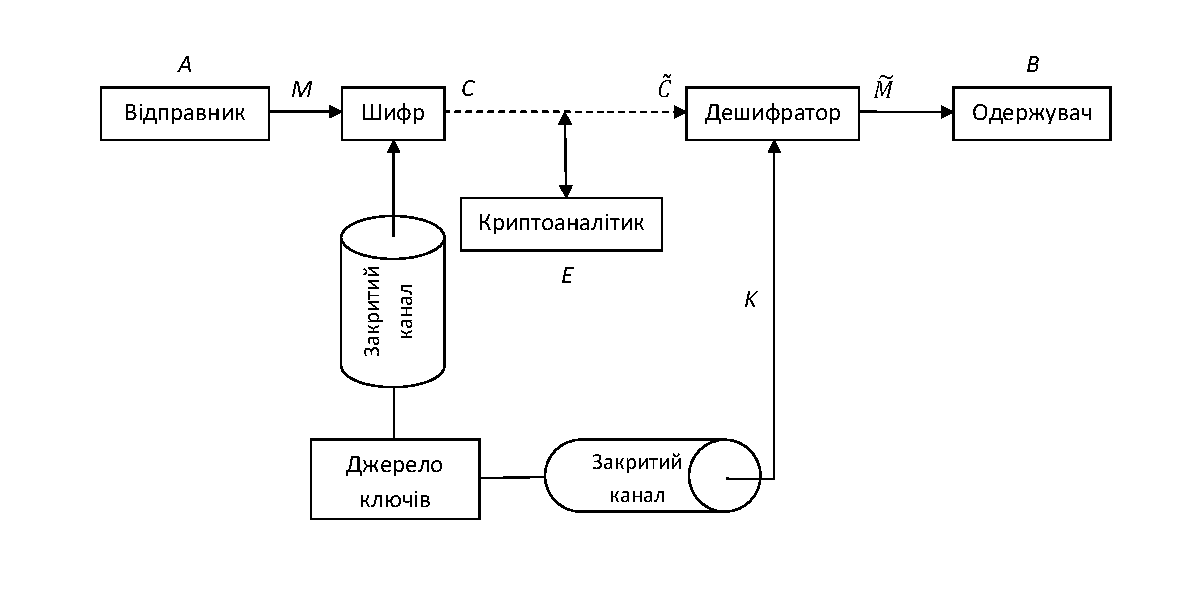
\includegraphics[width=\textwidth]{scheme}
\caption{Загальна схема секретного зв'язку}
\label{im:S_scheme}
\end{figure} 

На рисунку \ref{im:S_scheme}: \textsl{M, C} --
це власне відкритий і шифрований текст;
$\widetilde {M}, \widetilde{C}$ -- якісь змінені ВТ і ШТ відповідно, якщо криптоаналітик \textsl{E} вніс якісь зміни. Зауважимо, що в схемі Шеннона $\textsl {M} = \widetilde{M}$ і $\textsl {C} = \widetilde{C} $. Ну і звісно 
 \textsl{K} є закритим ключем. \par
Пунктирна лінія означає, що передача може бути припинена і передана інформація - змінена.

\begin{center}
Математична модель криптосистеми
\end{center}

З математичної точки зору, криптосистема є сукупністю просторів
\[ \Sigma =  \langle {\mathcal{M},\mathcal{C},\mathcal{K},\mathcal{E},\mathcal{D}} \rangle \, ,\]
\(
\begin{aligned}
\text{де } \mathcal{M} & - \text{простір відкритих текстів}, \\
\mathcal{C} & - \text{простір криптограм}, \\
\mathcal{K} & - \text{простір ключів}, \\
\mathcal{E}  & - \text{простір алгоритмів шифрування}, \\
\mathcal{D} &  - \text{простір алгоритмів розшифрування}.
\end{aligned}
\)  \\ \par
Далі будемо вважати, що $ E_k \in \mathcal{E} $ и $ D_k \in \mathcal{D} $ -- конкретні перетворення, тобто алгоритми шифрування і розшифрування на ключі \textsl {k} відповідно. \par
У загальному випадку під \textsl{шифром} визначається наступне:
\begin{equation}
\text{це відображення} \: \mathcal{M} \times \mathcal{K} \rightarrow \mathcal{C} : \forall{k} \in \mathcal{K}, \textsl{M} \in \mathcal{M} : D_k(E_k(\textsl{M}))=\textsl{M} ,
\end{equation}
 де $E_k : \mathcal{M} \rightarrow \mathcal{C}$ -- ін'єктивне відображення, яке дає можливість зашифрувати будь-який ВТ на ключі \textsl{k}, ну і відповідно при цьому, також відбувається однозначне розшифрування.

\begin{center}
Основні припущення Сіммонса
\end{center}

1. Атака криптоаналітика \textsl{E} здійснюється за допомогою ШТ. \\ \par
Криптоаналітик E хотів би обдурити \textsl {B}, пославши якусь іншу криптограму і щоб він подумав, що це йому відправив \textsl {A}. Якщо така дія вдається \textsl {E}, то вважається, що абонент \textsl {B} введений в оману. \\ \par
2. На декартовому добутку $ \mathcal{M} \times \mathcal {K} $ задано ймовірнісний розподіл. \\ \par

Тобто, така ймовірність \textsl{P(\textsl{M,K})} : $\forall{\textsl{M}} \in \mathcal{M}, \textsl{K} \in \mathcal{K}$ виконується наступне: \\
\[
\sum\limits_{M,K} P(\textsl{M,K}) =1, \;
\sum\limits_{M} P(\textsl{M,K}) = P(\textsl{K}), \;
\sum\limits_{K} P(\textsl{M,K}) = P(\textsl{M}).
\]

Згідно з правилом Керкгоффса, всі простори криптосистеми
$\Sigma$ і розподіл на $ \mathcal{M} \times \mathcal {K} $ вважаються відомими криптоаналітику. \\ \par

Подивимося, як же Сіммонс розвивав свою теорію далі. \\ \par

Він розглянув 2 типи атак: \\ \par
1. \textbf{Імітація}: Криптоаналітик \textsl {E} не очікує справжній ШТ від 
\textsl {A}, тобто не перехоплюючи, формує помилковий ШТ 
$\widetilde {C}$ і відправляє його \textsl {B}. \par
Атака з імітацією вважається успішною, якщо \textsl{B} вважає, що 
$ \widetilde{C} $ допустима криптограма від \textsl {A}, тобто 
$ \widetilde{M} $ -- ВТ, прийнятий за допустимий текст \textsl {A}, навіть якщо \textsl {B} пізніше відправив \\ШТ $ \textsl{C} = \widetilde{C} $. Тобто ця криптограма не розпізнана і в цьому випадку, якщо B був введений в оману, то незалежно від того який там був текст  -- помилковий чи правильний, все одно атака є успішною через те, що криптограма прийшла не в той час, коли відправляв \textsl {A} і відповідно висновки з отриманої криптограми будуть інші. Тому що важливо не тільки зміст криптограми, а й коли вона прийшла.

Позначимо ймовірність імітації :
\begin{equation}  \label{eq:PIM}  
P_{\text{ім}} = \max_{\widetilde{C} \in \mathcal{C}} P(\widetilde{C}- \text{допустима})
\end{equation}
Тобто, щоб обдурити \textsl{B}, криптоаналітик \textsl{E} намагається вибрати таку криптограму $ \widetilde {C} $, щоб максимізувати ймовірність \eqref{eq:PIM}. \\ \par
2. \textbf{Атака підміни}: \textsl{E} перехоплює справжній ШТ \textsl {C} 
від \textsl {A} і формує помилковий ШТ $ \widetilde{C} $ 
і передає його \textsl {B}. \par
Атака вважається успішною, якщо \textsl{B} прийняв $ \widetilde{C} $ за допустиму. \par
Позначимо ймовірність підміни:
\begin{equation}  \label{eq:PSUB}  
P_{\text{підм}} = \max_{\substack{\widetilde{C} \neq \textsl{C} \\
\widetilde{C} \in \mathcal{C}}} P(\widetilde{C} - \text{допустима})
\end{equation} 

Тоді ймовірність обману користувача \textsl{B} буде визначатися так: 
\begin{equation}  \label{eq:PLIE}  
P_{\text{об}} = \max\{P_{\text{ім}},P_{\text{підм}}\}
\end{equation} 

Як визначити систему, яка буде цілком таємною, тобто найкраща з точки зору криптостійкості. То тут цілком природньо було б визначити абсолютно автентичну криптосистему. Але як її визначити, тобто найкращу з точки зору неможливості підробки, обману або такої імітації, не зовсім зрозуміло. І це вже не зовсім тривіальне питання, тому що, якщо передається якесь повідомлення, то така ймовірність обману все одно буде, як ми незабором це побачимо. \\ \par

Проілюструємо загальну схему роботи криптосистеми
на малюнку \eqref {im:S_illustration}. \\
Розглянемо скінченну множину відкритих текстів \textsl{M}, яке зазвичай є певною підмножиною більшої множини і множину шифрованих текстів 
\textsl{C}, яке зазвичай більше за множину ВТ.
Також є множина ключів, яка практично збігається з усім простором ключів, за виключення нетипових слабких ключів. \par
Нехай обрані ключі $ K_1, K_2, K_3 $, на яких працюють абоненти. То ми можемо сказати, що весь простір ВТ відобразиться в деякий підпростір ШТ і позначимо їх $ C_1, C_2, C_3 $ відповідно, які в свою чергу можуть перетинатися, а можуть і не перетинатися.

\begin{figure}[h]
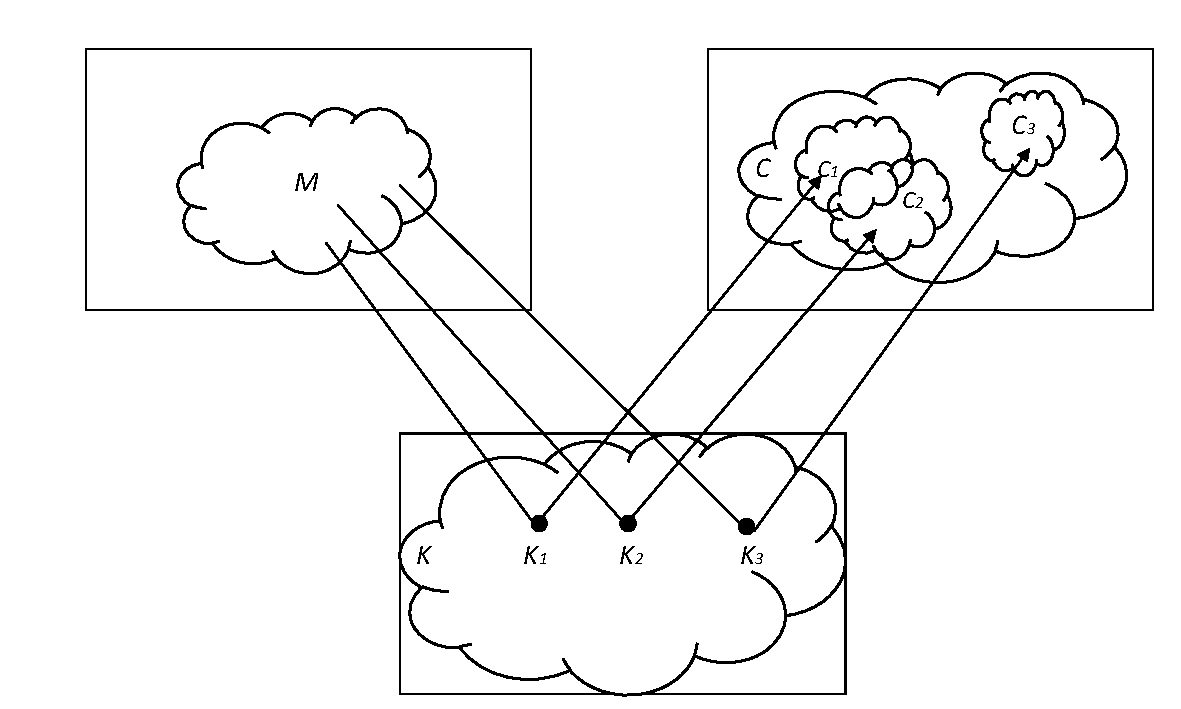
\includegraphics[height=8cm,width=\textwidth,]{illustration}
\caption{Ілюстрація загальної схеми секретного зв'язку}
\label{im:S_illustration}
\end{figure} 
\pagebreak

Розглянемо атаку імітації. \par
Нехай \textsl{A} і \textsl{B} працюють на ключі \textsl{k} і відповідно заданий алгоритм шифрування на цьому ключі:
$E_k(\mathcal{M})=\mathcal{C}_k$, де 
$\mathcal{C}_k \in \mathcal{C}, \textsl{k} \in \mathcal{K}$.   \par
Тоді, якщо абонентами \textsl{A} і 
\textsl{B} вибирається випадкове \textsl{k}, а криптоаналітиком \textsl{E} таке $\widetilde{C} \subset \mathcal{C} $ і відправляє $ \widetilde{C} \rightarrow \textsl{B} $, то ймовірність успіху атаки:
\begin{equation} \label{eq:PIM2}
P(\widetilde{C} - \text{допустима}) = 
\frac{|\mathcal{C}_k|}{|\mathcal{C}|} \geq \frac{|\mathcal{M}|}{|\mathcal{C}|} \textgreater 0,
\end{equation}
причому $|\mathcal{C}_k| \geq |\mathcal{M}| $ через однозначність розшифрування. Також ясно, що $ |\mathcal{M}| \textgreater 0 $. Ну і власне ймовірність \eqref{eq:PIM2} більше нуля, з чого і випливає, що така ймовірність обману існує. \par

В нерівності \eqref{eq:PIM2} досягається рівність $\Leftrightarrow$ 
$\forall \textsl{k} \in \mathcal{K}: |\mathcal{C}_k|=|\mathcal{M}|$, 
\\тобто $\forall{k} \in \mathcal{K}: E_k : \mathcal{M} \rightarrow \mathcal{C}_k$ -- бієкція. \par

Виникає питання, а як же зробити ймовірність обману меншою? \par
Коли застосовуємо до повідомлення цифровий підпис, то фактично ймовірність обману зменшується через те, що збільшується простір ШТ. Далі буде з'ясовано, яким чином вирішити це питання за допомогою імітовставок.

У загальному випадку \textsl{K} вибирається з ймовірністю $P(K)$. \par   
Позначимо через:

\[
        \Ind{K}(\textsl{C\,})=\begin{cases}
                1, &\text{якщо }  \textsl{C} \in \mathcal{C}_K \\
                0, &\text{якщо }  \textsl{C} \notin \mathcal{C}_K
        \end{cases}  - \text{індикатор } \textsl{C},
\] 
тобто $\Ind{K}(\textsl{C\,}) : \mathcal{C} \rightarrow \binsp{} $

Ймовірність того, що $ \widetilde{C} $ -- допустима, визначається наступним:

\begin{equation} \label{eq:P_ALLOWABILITY}
P(\widetilde{C} - \text{допустима}) = 
\sum\limits_{K \in \mathcal{K}} P(\textsl{K}) \cdot \Ind{K}(\widetilde{C})
\end{equation}

Ми не знаємо секретного ключа \textsl{K}, але ми знаємо його розподіл, через що у нас і буде визначена ймовірність \eqref {eq:P_ALLOWABILITY}. Тоді: 
\begin{equation} \label{eq:PIM3}
P_{\text{ім}} = \max_{\substack{\widetilde{C} \in \mathcal{C}}} P(\widetilde{C} - \text{допустима}) =
\max_{\substack{\widetilde{C} \in \mathcal{C}}} 
\sum\limits_{K \in \mathcal{K}} P(\textsl{K}) \cdot \Ind{K}(\widetilde{C}) 
\end{equation}

Шляхом деяких технічних міркувань, з використання нерівності Йєнсена, Сіммонс оцінив ймовірність \eqref{eq:PIM3}:

\begin{equation} \label{eq:P_EVALUATION}
P_{\text{ім}} \geq 2^{-I(\mathcal{C, K})} \:,
\end{equation}
де $I(\mathcal{C, K}) = H(\mathcal{C}) - H(\mathcal{C} | \mathcal{K}) $ -- взаємна інформація. 

При цьому, в нерівності \eqref{eq:P_EVALUATION} рівність досягається 
$\Leftrightarrow$ виконуються наступні умови: \par
1. $P(\widetilde{C} - \text{допустима})$ не залежить від $\widetilde{C}$. Тобто оптимальна атака -- це випадковий вибір криптограми 
$\widetilde{C}$. \par
2. $P(\widetilde{C} | \textsl{K})$ однакова для $\forall \textsl{K} \in \mathcal{K} : \widetilde{C} \in \mathcal{C}_K $, тобто $\Ind{K}(\widetilde{C}) = 1.$

Тоді ймовірність обману визначається наступним:
\begin{equation} \label{eq:PLIECOMMON}
P_{\text{об}} = \max\{P_{\text{ім}},P_{\text{підм}}\} \geq 2^{-I(\mathcal{C, K})} \,.
\end{equation}

\begin{mydef} 
Абсолютно автентичною криптосистемою називається така, для якої в нерівності \eqref{eq:PLIECOMMON} досягається рівність.
\end{mydef}

Ймовірність \eqref{eq:PLIECOMMON} не може бути нульовою, але вона може бути мінімізована, коли взаємна інформація між $ \mathcal{C} $ і 
$ \mathcal{K}$ в свою чергу максимізована. Трактується це наступним чином: наскільки ключ використовується для створення умов імітостійкості. \\ \par

\begin{example}
$\mathcal{M} = \{M_1, M_2\}$ , 
$\mathcal{K} = \{K_1, K_2\}$, 
%$P(K_1) = P(K_2) = \frac{1}{2}, P(M_1) = P(M_2) = \frac{1}{2}$
де кожна подія приймається з однаковою ймовірністю. 
$\mathcal{C}$ = \{00, 01, 10, 11\}.
\end{example} \par  
Задамо алгоритм шифрування у вигляді таблиці \eqref{tab:T1}, при якому показано, якому ШТ відноситься відповідний ВТ на заданому ключі. Також ми подивимось, чи можна зробити ймовірність імітації рівній
 $ \frac{1}{2} $ і яка ж буде ймовірність обману. \\ \par
\begin{wraptable}{l}{0.22\linewidth}
\begin{tabular}{|c||c|c|}\hline
\backslashbox{K}{M}
&\makebox[1.5em]{$M_1$}&\makebox[1.5em]{$M_2$} \\\hline\hline
$K_1$  &00&10 \\ \hline
$K_2$  &01&11 \\ \hline 
\end{tabular} 
        \caption{Алгоритм шифрування}
        \label{tab:T1}
\end{wraptable} 
Однозначність розшифрування в даному прикладі забезпечена, так як видно, що при кожному ключі - ВТ переходить в якийсь відмінний від інших ШТ. \par
Знайдемо взаємну інформацію між $\mathcal{C}$ і $\mathcal{K}$ :
 \begin{equation}
 I(\mathcal{C}, \mathcal{K}) = H(\mathcal{C}) - H(\mathcal{C} | \mathcal{K}) =
  \log(4) - \log(2) = 1 
 \end{equation} 
  
Якщо криптоаналітик посилає якусь довільну криптограму і якщо \textsl{А} і \textsl {B} працюють на ключі $ \textsl{K}_1 $, то він завжди обдурить, якщо вибере один з двох ШТ: 00 або 10. Тобто він з ймовірністю 
$\frac{1}{2}$ зможе здійснити атаку імітації і таким чином в нерівності 
\eqref{eq:P_EVALUATION} досягається рівність. \par
Але чому ж дорівнює ймовірність підміни? \par
Можна помітити, що якщо ключ $ \textsl{K}_1 $, то в криптограмі останній біт -- 0, на ключі $ \textsl{K}_2 $, відповідно -- 1. Таким чином, ми по криптограмі можемо зрозуміти на якому ключі працюють \textsl{А} і 
\textsl{B}, і фактично ця система з точки зору стійкості -- погана. 
Тоді ймовірність підміни буде дорівнювати одиниці, через наступний фактор. Якщо ми перехопимо криптограму 00, то зразу посилаємо 10 і навпаки. 
Ну і звичайно ж ймовірність обману строго більше $  \frac{1}{2} $, 
тобто в \eqref{eq:PLIECOMMON} рівність не досягається. \par
З усього цього слідує те, що наш шифр не є абсолютно автентичним.
Ну і звичайно ж зрозуміло, щоб зменшити ймовірність підміни, необхідно розширювати простір ШТ.
Для цих цілей використовують імітовставки.
\begin{center}
Імітовставки
\end{center}

Нехай $ \textsl{E}_K $ -- алгоритм блочного шифру, а повідомлення 
\textsl{M} розбивається на блоки, \\
тобто $ M = M_1 M_2 \dots M_t $ і в режимі зчеплення блоків при таємному ключі \textsl{K} знаходимо
\begin{equation}
H_i = E_K(M_i \xor H_{i-1}) \:, i=\overline{1,t}
\end{equation}

Розмір блоку дорівнює розміру входу і виходу. тобто
$ |M_i | = |E_K(X)| = |X| $, відповідно \\
$ H_0 $ - вектор ініціалізації, а $ H_t $ - імітовставка. \par
Повідомлення з імітовставкою $ (M, H_t) $ забезпечує автентичність з 
використанням секретного ключа, і при цьому простір отриманих текстів 
розширюється і далі воно може бути зашифровано іншим ключем. Для цієї мети 
також використовуються геш-функції із секретним ключем -- $h(X,K)$.  
\\ \par
Властивості $h(X,K)$:
\begin{enumerate}
\item[1)] Швидке обчислення.
\item[2)] $ \forall M \in \mathcal{M} $ не можна вгадати значення 
геш-функції $h(M,K)$ з ймовірністю більш ніж $ 2^{\min\{m,|K|\}} $, 
де $|K|$ -- довжина ключа в бітах, $m$ -- розмір виходу $h(X,K)$.
\item[3)] Для скінченного набору: $ \{M_i, h(M_i, k) \}_ {i = 1}^ t $ не можливо знайти хоча б одну пару
 $ (M, \widetilde{M}) \: \text {:} \: H(M, k) = h(\widetilde {M}, k) \text{,}\: M \neq \widetilde {M} $ за поліноміальний час.
 
\end{enumerate}
 
Приклад геш-функцій з ключем: імітовставки.

          % 11
\section{Iдентифікація та автентифікація. Криптографічні протоколи аутентифікації}
\begin{flushright}
\emph{(Автор: Марина Соловйова. Частково редагувалось.)}
\par \emph{(Версія від 22 січня 2017 р.)}
\end{flushright}

\par\emph{Ідентифікація} - це надання суб'єкту (об'єкту) індивідуального кода (наприклад, номера), тобто ідентифікатора, який відрізняється від всіх інших, а також перевірка ідентифікатора(все це не секретні дані). \par
\emph{Автентифікація} - це перевірка достовірності суб'єкту по наданим ідентифікаторам та деякій додатковій інформації (наприклад, паролям, ключам) шляхом порівняння.
\parПри контакті користувача, наприклад, з комп'ютерною мережею здійснюються наступні процедури:

\begin{itemize}
\item ідентифікація
\item автентифікація
\item авторизація
\end{itemize}

\begin{center}
\textbf{Принципи аутентифікації}
\end{center}

\begin{enumerate}
\setcounter{enumi}{0}
\item По наданню деякої секретної інформації, відомої користувачеві (пароль, код).
\item По наданню деяких об'єктивних характеристик (мікросхема, магнітна стрічка).
\item По наданню індивідуальних біометричних характеристик (відбитків пальців, рисунку райдужної оболонки ока, тембру голосу).
\item По характеристикам роботи з апаратурою в реальному часі.
\item По відповідям в режимі діалогу.
\item За допомогою третьої сторони.
\end{enumerate}

\begin{center}
\textbf{Криптографічні протоколи аутентифікації}
\end{center}

\begin{enumerate}
\item Автентифікація за допомогою пароля  (на прикладі аутентифікації з комп'ютерною системою -- надалі будемо позначати як <<КС>>).
 \begin{enumerate}
    \item \textit{Парольна автентифікація з використанням односторонніх функцій}
    \parНехай h(x) -- одностороння хеш-функція, що володіє сильною стійкістю до колізій.
    \parКористувачі $A_{i}$ мають ідентифікатори $D_{i}$ та паролі $p_{i}$, i = $\overline{1,n}$.

\begin{enumerate}       
        \item Попередньо в КС формується та розміщується табличка \newline T = $\{D_{i}, H_{i}, i = \overline{1,n}\}$, де $H_{i} = h(p_{i},D_{i})$.
        \item (При контакті) $A_{i}: (p_{i},D_{i}) \rightarrow $ КС.
        \item КС перевіряє: ?$D_{i} \in T$? (ідентифікація),
        \item ?$h(p_{i}, D_{i}) = H_{i}? \longleftrightarrow ?H_{i} \in T$? (автентифікація).
        \item Якщо все виконується, то авторизація, інакше - відмова.  
\end{enumerate}
   
    \item \textit{Паралельна автентифікація за допомогою симетричного шифрування стійких до атак на основі відкритого тексту (ВТ).}
     \parКористувачі $A_{i}$ мають ідентифікатори $D_{i}$ та паролі $p_{i}$, $i = \overline{1,n}$.
     \parНехай $E_{k}$ - алгоритм симетричного шифрування, стійкий до атак на основі ВТ.
     
\begin{enumerate}
     \item Попередньо в КС формується та розміщується табличка 
     \item T = $\{D_{i}, C_{i}, i = \overline{1,n}\}$, де $C_{i} = E_{p_{i}}(D_{i})$.
     \item $A_{i}: (p_{i},D_{i}) \rightarrow $ КС.
     \item КС перевіряє: ?$D_{i} \in T$? та ?$E_{p_{i}}(D_{i}) = C_{i}$?
     \newline Якщо все виконується, то авторизація, інакше -- відмова.
\end{enumerate}

    \item \textit{Парольна автентифікація з захистом від коротких паролів.}
\begin{enumerate}
     \item модифікація в варіанті 1 з хеш-функцією h(x) - використання односторонніх хеш-функцій з секретним ключем (який відомий лише адмін-у КС).
     \item модифікація в варіанті 2: табличка T = $\{D_{i}, C_{i}, i = \overline{1,n}\}$ - використання секретного ключа k: $C_{i} = E_{p_{i}\oplus k}(D_{i})$.
     \newlineПеревірка аналогічна.
\end{enumerate}    
    
    \item \textit{Парольна автентифікація зі змінним паролем.}
    \par Користувачі $A_{i}$ мають ідентифікатори $D_{i}$ та паролі $p_{i}^{(0)}, i = \overline{1,n}$.
    \newline Наявна одностороння стійка до колізій хеш-функція h(x) (відкрита).
\begin{enumerate}
    \item Кожен $A_{i}$ обчислює ряд разових паролів: 
    \[
    p_{i}^{(0)}, p_{i}^{(1)} = h(p_{i}^{(0)}), p_{i}^{(2)} = h(p_{i}^{(1)}) = h^{2}(p_{i}^{(0)}) \vdots p_{i}^{(t)} = h^{t}(p_{i}^{(0)}) \: \text{та} \: p_{i}^{(t)} \rightarrow  \text{КС}, 
    i = \overline{1,n}.
    \]
    \item КС формує табличку T = $\{D_{i}, p_{i}^{(t)}, i = \overline{1,n}\}$.
    \item (При контакті) $A_{i}: (D_{i}, p_{i}^{(t-1)}) \rightarrow $ КС.
    \item КС перевіряє: ?$D_{i} \in T$? та ?$h(p_{i}^{(t-1)}) = p_{i}^{(t)}$?
    \newline Якщо все в виконується, то виконується авторизація і КС в табличці T змінює $(D_{i}, p_{i}^{(t)})$ на $(D_{i}, p_{i}^{(t-1)})$.
    \item (При другому контакті) $A_{i}: (D_{i}, p_{i}^{(t-2)}) \rightarrow $ КС.
    \item КС перевіряє: ?$D_{i} \in T$? та ?$h(p_{i}^{(t-2)}) = p_{i}^{(t-1)}$? 
\end{enumerate}   
   Якщо все виконується, то КС в табличці T змінює $(D_{i}, p_{i}^{(t-1)})$ на $(D_{i}, p_{i}^{(t-2)})$.
    \newline \textbf{\textit{Примітка:}} Якщо всі разові паролі будуть вичерпані, потрібно згенерувати нові їх послідовності.
    \newline Але що робити при технічному збої? Зрозуміло, що повторювати пароль не можна. Тому при, наприклад, однократному збої на кроці 6):
    $A_{i}: (D_{i}, p_{i}^{(t-3)}) \rightarrow $ КС. Після чого КС перевіряє: ?$D_{i} \in T$? та ?$h^{2}(p_{i}^{(t-3)}) = p_{i}^{(t-1)}$? після чого алгоритм продовжує свою роботу.
 \end{enumerate} 
 
 \item Автентифікація за допомогою симетричних криптосистем.
  \parКористувачі $A_{i}$, $i = \overline{1,n}$ мають ідентифікатори $D_{i}$ та $K_{ij}$ - секретні ключі $A_{i}$ та $A_{j}$ зі спільною системою симетричного шифрування $(E_{k}, D_{k})$.
  \begin{enumerate}
  
  \item Ініціатор аутентифікації $A_{i}: D_{i} \rightarrow A_{j}$.
  \item $A_{j}$ генерує випадкове $M \rightarrow A_{i}$.
  \item $A_{i}$ шифрує на спільному ключі повідомлення: $E_{K_{ij}}(M) = C_{ij} \rightarrow A_{j}$.
  \item $A_{j}$ перевіряє: $D_{K_{ij}}(C_{ij}) = M$.
  \end{enumerate}
  
 \item Автентифікація за допомогою асиметричних криптосистем (на прикладі RSA).
  \parКористувачі $A_{i}$, $i = \overline{1,n}$ мають відкриті $(n_{i}, e_{i})$ та закриті $d_{i}$ ключі RSA.
 \begin{enumerate}
   \item За допомогою цифрового підпису (ЦП).
  
   \begin{enumerate}
   \item $A_{i}$ генерує випадкове М і підписує його, тобто:
   \newline $S = M^{d_{i}}mod$ $n_{i}$, $\Rightarrow  (M, S) \rightarrow A_{j}$.
   \item $A_{j}$ перевіряє ЦП: ?$S^{e_{i}}mod \:n_i= M$?
   \item За допомогою шифрування.
   \end{enumerate}

 \end{enumerate}
 \item Автентифікація за допомогою протоколу доказу без розголошення.
\end{enumerate}          % 12
%\input{}       % 13
%\input{}       % 14
%\input{}       % 15
%\input{}       % 16
%\input{}       % 17
%\input{}       % 18
\section{Lecture 13}
\section{Lecture 14}
\section{Lecture 15}
\section{Lecture 16}
\section{Lecture 17}
\section{Lecture 18}



\end{document}

